\documentclass[12pt,a4paper]{report}
\usepackage{graphicx}
\usepackage{tikz}
\usepackage[utf8]{inputenc}
\usepackage[T1]{fontenc}
\usepackage[french]{babel}
\usepackage{lmodern}
\usepackage{geometry}
\usepackage{setspace}
\usepackage{graphicx}
\usepackage{float}
\usepackage{booktabs}
\usepackage{longtable}
\usepackage{tabularx}
\usepackage{array}
\usepackage{hyperref}
\usepackage{microtype}
\usepackage{pdflscape}

\geometry{left=2.5cm,right=2.5cm,top=2.5cm,bottom=2.5cm}
\onehalfspacing
\setlength{\parindent}{0.8cm}
\setlength{\parskip}{0.2cm}
\graphicspath{{figures/}}
\hyphenpenalty=10000
\exhyphenpenalty=10000
\tolerance=2000
\emergencystretch=3em

\hypersetup{
  colorlinks=false,
  pdftitle={Rapport PFA Tastify},
  pdfauthor={Diouri Mehdi et El kherazi Ibtihal}
}

\newcolumntype{Y}{>{\raggedright\arraybackslash}X}
\newcommand{\code}[1]{\texttt{#1}}
\newcommand{\pathcode}[1]{{\scriptsize\path{#1}}}
\newcommand{\placeholder}[1]{\textit{#1}}

\newcommand{\schemaNode}[1]{\fbox{\begin{minipage}{0.18\textwidth}\centering\small #1\end{minipage}}}
\newcommand{\schemaArrow}{\quad$\longrightarrow$\quad}

\begin{document}

\pagenumbering{Alph}
\begin{titlepage}

\begin{tikzpicture}[remember picture,overlay]
\fill[green!70!black] ([xshift=1.15cm]current page.north west) rectangle ([xshift=1.45cm]current page.south west);
\fill[red!70!black] ([xshift=1.15cm,yshift=0.8cm]current page.south west) rectangle ([xshift=1.45cm]current page.south west);
\end{tikzpicture}

\begin{center}

\vspace*{-0.7cm}

% Logos
\begin{minipage}{0.42\textwidth}
\centering

\includegraphics[width=\textwidth]{logo_emsi.png.png}
\end{minipage}
\hspace{1.1cm}
\begin{minipage}{0.29\textwidth}
\centering

\includegraphics[width=\textwidth]{honoris logo.jpg}
\end{minipage}

\vspace{3.2cm}

% Titre principal
{\Huge \textbf{Rapport de Projet Fin d'Année}}

\vspace{1.8cm}

% Sujet du projet
{\large \textbf{Application ERP de gestion de restaurant}}

\vspace{0.15cm}

{\large \textbf{Analyse de sentiment des avis clients et pilotage opérationnel}}

\vspace{1.7cm}

% Année universitaire
{\LARGE \textbf{Année Universitaire :}}

\vspace{0.15cm}

{\LARGE \textbf{2025 -- 2026}}

\end{center}

\vspace{2.3cm}

% Réalisé par
\begin{flushleft}
\hspace{1.45cm}\textbf{Réalisé par :}

\vspace{0.15cm}

\hspace{1.45cm}DIOURI Mehdi

\hspace{1.45cm}EL KHARRAZI Ibtihal
\end{flushleft}

\vspace{0.65cm}

% Encadré par
\begin{flushleft}
\hspace{1.45cm}\textbf{Encadré par :}

\vspace{0.15cm}

\hspace{1.45cm}Mme. BENSALEH Nouhaila
\end{flushleft}

\end{titlepage}
\newpage
\thispagestyle{empty}
\null
\newpage


\clearpage
\pagenumbering{roman}

\chapter*{Dédicaces}
\addcontentsline{toc}{chapter}{Dédicaces}
Nous dédions ce travail à nos familles, qui nous ont soutenus tout au long de ce projet. Leur patience, leur confiance et leurs encouragements nous ont aidés à avancer, surtout pendant les périodes les plus chargées.

Nous le dédions aussi à nos enseignants, pour les connaissances qu’ils nous ont transmises en génie logiciel, développement web, bases de données, modélisation, sécurité et gestion de projet.

Enfin, nous pensons à toutes les personnes qui nous ont encouragés à apprendre par la pratique, à corriger nos erreurs et à progresser étape par étape.

\chapter*{Remerciements}
\addcontentsline{toc}{chapter}{Remerciements}
Avant de présenter le projet Tastify, nous tenons à remercier nos familles pour leur soutien tout au long de notre formation. Leur présence et leurs encouragements nous ont aidés à avancer avec sérieux jusqu’à la réalisation de ce Projet de Fin d’Année.

Nous remercions aussi l’ensemble du personnel enseignant et administratif pour le cadre de travail qu’il nous a offert durant cette année.

Nous adressons un remerciement particulier aux enseignants qui nous ont accompagnés dans les matières liées à ce projet : conception UML, développement backend, développement frontend, architecture logicielle, bases de données, tests et documentation technique. Les connaissances acquises dans ces modules nous ont permis de concevoir et de réaliser Tastify dans de bonnes conditions.

\chapter*{Résumé}
\addcontentsline{toc}{chapter}{Résumé}
Tastify est une application web full-stack destinée à centraliser la gestion quotidienne d'un restaurant. Le projet répond à des difficultés concrètes observées dans la restauration : dispersion des informations, erreurs de transmission entre la salle et la cuisine, suivi manuel des stocks, manque de visibilité sur les réservations, encaissements complexes et exploitation limitée des avis clients.

La solution repose sur un backend Django REST Framework, une base de données MySQL, Redis pour les échanges temps réel et les traitements asynchrones, Celery pour les tâches de fond, ainsi que deux applications React : une interface staff pour le gérant, le serveur et le cuisinier, et un portail client. Les modules réalisés couvrent le menu, les tables, les commandes, le Kitchen Display System, les stocks, les ressources humaines, les réservations, les paiements, la fidélité, les avis, les tableaux de bord et la configuration du restaurant.

Une partie importante du projet concerne l'analyse de sentiment des avis clients. Le code implémente un pipeline asynchrone qui analyse les commentaires au moyen de l'API Hugging Face lorsque le jeton est configuré. Il utilise le modèle multilingue NLP Town pour les avis non arabes, MARBERT pour les commentaires en arabe, et un secours local par mots-clés nommé \pathcode{mots-cles-simple}. Les identifiants exacts des modèles sont détaillés dans le chapitre consacré à l'analyse de sentiment. Cette fonctionnalité aide le gérant à suivre la satisfaction client sans interrompre l'expérience utilisateur.

\textbf{Mots-clés :} ERP, restaurant, Django, React, MySQL, Redis, Celery, WebSocket, KDS, avis clients, analyse de sentiment, Hugging Face, PFA.


\chapter*{Liste des abréviations}
\addcontentsline{toc}{chapter}{Liste des abréviations}
\begin{longtable}{p{3cm}p{11cm}}
\toprule
\textbf{Abréviation} & \textbf{Signification} \\
\midrule
\endfirsthead
\toprule
\textbf{Abréviation} & \textbf{Signification} \\
\midrule
\endhead
API & Application Programming Interface. \\
ASGI & Asynchronous Server Gateway Interface. \\
CRUD & Create, Read, Update, Delete. \\
DRF & Django REST Framework. \\
ERP & Enterprise Resource Planning, progiciel de gestion intégré. \\
JWT & JSON Web Token. \\
KDS & Kitchen Display System, écran de suivi des commandes en cuisine. \\
ML & Machine Learning, apprentissage automatique. \\
NLP & Natural Language Processing, traitement automatique du langage naturel. \\
ORM & Object-Relational Mapping. \\
PFA & Projet de Fin d'Année. \\
PWA & Progressive Web App. \\
RBAC & Role-Based Access Control, contrôle d'accès basé sur les rôles. \\
REST & Representational State Transfer. \\
SPA & Single Page Application. \\
SQL & Structured Query Language. \\
UML & Unified Modeling Language. \\
WS & WebSocket. \\
\bottomrule
\end{longtable}


\tableofcontents
\listoffigures
\listoftables

\cleardoublepage
\pagenumbering{arabic}

\chapter*{Introduction générale}
\addcontentsline{toc}{chapter}{Introduction générale}

La transformation numérique des restaurants ne se limite plus à la présence en ligne ou à la prise de réservation. Elle concerne désormais l'organisation opérationnelle dans son ensemble : coordination entre la salle et la cuisine, disponibilité des plats, suivi des stocks, gestion des paiements, fidélisation et analyse des retours clients. Dans un établissement où plusieurs acteurs interviennent simultanément, une information mal transmise peut entraîner un retard, une erreur de préparation, une rupture non anticipée ou une dégradation de l'expérience client.

Le projet Tastify s'inscrit dans ce contexte. Il propose une application web centralisée pour la gestion d'un restaurant, en couvrant à la fois les besoins internes du personnel et les interactions avec les clients. La solution s'appuie sur une architecture full-stack composée d'un backend Django REST Framework, d'une base de données MySQL, de Redis et Celery pour les échanges temps réel et les traitements asynchrones, de Django Channels pour les WebSocket, ainsi que de deux applications React : une interface staff et un portail client.

La particularité du projet réside dans son périmètre transversal. Tastify ne se limite pas à un module de menu ou à une caisse numérique : il relie les tables, les commandes, le Kitchen Display System, les stocks, les réservations, les paiements, la fidélité, les avis clients et les tableaux de bord. Cette intégration rend le projet pertinent dans le cadre d'un Projet de Fin d'Année, car elle mobilise plusieurs dimensions du génie logiciel : modélisation, architecture, API, sécurité, temps réel, asynchronisme, expérience utilisateur et validation.

Le présent rapport est organisé selon une progression académique classique. Le premier chapitre présente le contexte général, la problématique, l'étude de l'existant et les objectifs. Le deuxième chapitre formalise l'analyse des besoins et la conception. Un chapitre spécifique est consacré à l'analyse de sentiment, car cette fonctionnalité combine un enjeu métier et un pipeline technique précis. Les chapitres suivants décrivent l'architecture, la réalisation, les interfaces, les tests, les limites et les perspectives.

La rédaction adopte enfin un principe de rigueur : les fonctionnalités sont présentées lorsqu'elles sont effectivement intégrées au périmètre du projet, tandis que les limites et les éléments restant à compléter sont explicitement distingués. Cette approche permet de défendre le travail réalisé sans surestimer son niveau de maturité.

\chapter{Contexte général}
\label{chap:contexte}

\section*{Introduction}
\addcontentsline{toc}{section}{Introduction}
Ce chapitre place Tastify dans son contexte métier. Il décrit les problèmes rencontrés dans la gestion d'un restaurant, formule la problématique, compare quelques solutions existantes et fixe les objectifs retenus pour le projet.

\section{Contexte métier}
Un restaurant fonctionne avec des enchaînements rapides. Une table se libère, un serveur prend une commande, la cuisine prépare les plats, le stock diminue, le paiement est enregistré, puis le client peut laisser un avis. Chaque étape dépend de la précédente, et plusieurs rôles interviennent en même temps : gérant, serveur, cuisinier et client.

Quand ces informations sont réparties entre plusieurs outils, les erreurs arrivent vite. Un serveur peut annoncer un plat qui n'est plus disponible. La cuisine peut recevoir une commande incomplète. Le gérant peut découvrir une rupture de stock après le service. Les avis clients peuvent rester dispersés et ne servir à aucune décision. Une application utile doit donc réunir ces informations au même endroit et réduire les pertes de temps entre les acteurs.

\section{Problématique}
La problématique principale du projet peut être formulée de cette manière :

\begin{quote}
Comment concevoir une application web centralisée, maintenable et accessible permettant de gérer les opérations d'un restaurant, tout en améliorant la coordination entre la salle, la cuisine, la gestion administrative et l'expérience client ?
\end{quote}

Cette problématique conduit à plusieurs questions concrètes :

\begin{itemize}
  \item comment séparer les accès selon les rôles sans multiplier les applications inutilement ;
  \item comment envoyer rapidement les commandes vers la cuisine ;
  \item comment relier commandes, stocks, paiements et fidélité ;
  \item comment analyser les avis clients sans ralentir l'expérience utilisateur ;
  \item comment garder une architecture claire, testable et simple à déployer.
\end{itemize}

\section{Étude de l'existant}
Le marché propose déjà plusieurs solutions de caisse ou de gestion de restaurant. Elles couvrent souvent une partie du besoin : prise de commande, paiement, gestion des stocks ou reporting. Le tableau~\ref{tab:existant} résume leur positionnement par rapport à Tastify.

\begin{table}[H]
\centering
\caption{Comparaison synthétique des solutions existantes}
\label{tab:existant}
\begin{tabularx}{\textwidth}{p{2.8cm}YYY}
\toprule
\textbf{Solution} & \textbf{Points forts} & \textbf{Limites fréquentes} & \textbf{Lecture pour Tastify} \\
\midrule
Lightspeed Restaurant & Caisse, menu, commandes, reporting. & Coût récurrent, dépendance à une offre commerciale. & Confirme l'intérêt d'une solution intégrée. \\
Toast POS & Orientation restaurant, commande et paiement. & Disponibilité et adaptation au marché local variables. & Montre l'importance du lien salle-cuisine. \\
Revel Systems & Couverture ERP large, gestion multi-sites. & Coût et complexité élevés pour une petite structure. & Justifie un périmètre modulaire. \\
L'Addition & Solution spécialisée restauration, caisse et service. & Couverture variable selon les offres et les intégrations. & Sert de repère pour les besoins terrain. \\
Tastify & Projet web modulaire, deux portails, temps réel, avis et fidélité. & Prototype académique, pas de données de production. & Adapté au cadre pédagogique du PFA. \\
\bottomrule
\end{tabularx}
\end{table}

Cette comparaison montre que les solutions commerciales sont puissantes, mais qu'elles peuvent être coûteuses, fermées ou liées à un matériel précis. Tastify se place dans une logique pédagogique : comprendre les flux d'un restaurant, les modéliser proprement et proposer une architecture réutilisable.

\section{Objectifs du projet}
Les objectifs du projet sont les suivants :

\begin{itemize}
  \item centraliser la gestion des menus, catégories, plats, tables, commandes et réservations ;
  \item proposer une interface staff adaptée au gérant, au serveur et au cuisinier ;
  \item proposer un portail client pour consulter le menu, réserver, payer et suivre la fidélité ;
  \item améliorer la coordination cuisine avec un Kitchen Display System et des WebSocket ;
  \item gérer les stocks, les ingrédients, les recettes et les mouvements associés ;
  \item analyser les avis clients avec un traitement de sentiment lancé en arrière-plan ;
  \item obtenir une architecture testable, documentée et déployable avec Docker Compose.
\end{itemize}

\section{Périmètre fonctionnel retenu}
L'implémentation couvre les modules listés dans le tableau~\ref{tab:perimetre}.

\begin{table}[H]
\centering
\caption{Périmètre fonctionnel confirmé}
\label{tab:perimetre}
\begin{tabularx}{\textwidth}{p{3.2cm}Y}
\toprule
\textbf{Domaine} & \textbf{Fonctions couvertes} \\
\midrule
Menu & Catégories, plats, images, disponibilité et liens avec les ingrédients. \\
Salle & Tables, plan de salle, statut de table et prise de commande. \\
Cuisine & KDS, lignes de commande, statuts de préparation et synchronisation temps réel. \\
Stock & Ingrédients, seuils d'alerte, recettes et mouvements de stock. \\
RH & Employés, shifts, offres d'emploi et candidatures. \\
Réservations & Création, disponibilité, conflits de créneaux et gestion côté client/staff. \\
Paiements & Paiement d'une commande, contribution par ligne et lien avec le client. \\
Fidélité & Profil, points, transactions et récompenses. \\
Avis & Commentaires, note optionnelle et analyse de sentiment. \\
Analytics & Indicateurs de tableau de bord et statistiques de sentiment. \\
Configuration & Informations du restaurant, devise, couleurs, paramètres de service. \\
\bottomrule
\end{tabularx}
\end{table}

\section{Planification}
La planification ci-dessous synthétise les principales phases suivies durant le projet, à partir des modules livrés, des étapes de conception, des développements réalisés et des validations effectuées.

\begin{table}[H]
\centering
\caption{Planification pédagogique du projet}
\label{tab:planification}
\begin{tabularx}{\textwidth}{p{2.2cm}Yp{2.4cm}}
\toprule
\textbf{Phase} & \textbf{Contenu} & \textbf{Durée indicative} \\
\midrule
Phase 1 & Initialisation du dépôt, environnement Docker, modèles principaux, authentification et rôles. & 2 semaines \\
Phase 2 & Modules gérant : menu, catégories, stocks, ressources humaines et configuration. & 2 semaines \\
Phase 3 & Salle et cuisine : tables, commandes, KDS, statuts et WebSocket. & 2 semaines \\
Phase 4 & Portail client : menu public, réservation, compte, panier et paiement. & 2 semaines \\
Phase 5 & Fidélité, avis, analyse de sentiment et indicateurs analytics. & 2 semaines \\
Phase 6 & Tests, documentation, conteneurisation et préparation du rapport. & 1 semaine \\
\bottomrule
\end{tabularx}
\end{table}

\section{Méthodologie de travail}
Le projet a été conduit par itérations successives afin de garder un lien constant entre les besoins métier, la conception et l'implémentation. Chaque phase a produit un résultat vérifiable : modèle de données, API, écran React, scénario de test ou élément documentaire.

\begin{table}[H]
\centering
\caption{Méthodologie suivie pendant le projet}
\label{tab:methodologie-travail}
\begin{tabularx}{\textwidth}{p{3cm}Y}
\toprule
\textbf{Phase} & \textbf{Travail réalisé} \\
\midrule
Cadrage & Analyse du besoin restaurant, identification des acteurs, choix du périmètre et comparaison avec des solutions existantes. \\
Conception & Modélisation UML, découpage des modules Django, définition des routes API et organisation des deux applications React. \\
Réalisation backend & Implémentation des modèles, serializers, vues DRF, permissions, WebSocket, tâches Celery et services métier. \\
Réalisation frontend & Construction du back-office staff et du portail client avec React, Vite, TypeScript et Tailwind CSS. \\
Intégration & Connexion des frontends aux API, orchestration Docker Compose, synchronisation salle-cuisine et validation des flux de bout en bout. \\
Validation & Exécution des tests pytest, Vitest et Playwright, capture des interfaces, correction documentaire et préparation du rapport final. \\
\bottomrule
\end{tabularx}
\end{table}

Les outils utilisés ont structuré le travail quotidien : Git pour suivre l'évolution du code, Docker Compose pour lancer l'environnement complet, Django REST Framework pour l'API, React et Vite pour les interfaces, MySQL pour la persistance, Redis et Celery pour le temps réel et les traitements asynchrones, puis pytest, Vitest et Playwright pour la validation.

Les principales difficultés ont concerné la séparation claire des rôles, la synchronisation entre la salle et la cuisine, la cohérence entre paiements, commandes et fidélité, ainsi que la production d'un rapport fidèle au projet réel. Ces points ont été traités par un découpage modulaire, des tests ciblés et une documentation progressive des décisions.

\section{Répartition du travail}
La répartition a combiné spécialisation technique et validation croisée. Mehdi s'est concentré sur le socle backend, l'intégration, les tests et le déploiement. Ibtihal s'est concentrée sur les interfaces, l'expérience utilisateur, la documentation, les diagrammes UML et la validation fonctionnelle.

\begin{table}[H]
\centering
\caption{Répartition synthétique des contributions}
\label{tab:repartition-travail}
\begin{tabularx}{\textwidth}{p{2.7cm}YY}
\toprule
\textbf{Membre} & \textbf{Tâches réalisées} & \textbf{Contribution principale} \\
\midrule
Mehdi & Backend Django/DRF, modèles métier, API, authentification JWT, permissions, Redis, Celery, Docker Compose, tests pytest, intégration et préparation des résultats de validation. & Fiabilisation du cœur applicatif, cohérence des modules métier et validation technique. \\
Ibtihal & Frontends React staff et client, parcours utilisateur, interfaces UI, documentation du rapport, diagrammes UML, captures fonctionnelles et validation des scénarios métier. & Qualité de l'expérience utilisateur, lisibilité documentaire et cohérence fonctionnelle. \\
\bottomrule
\end{tabularx}
\end{table}

\section*{Conclusion}
\addcontentsline{toc}{section}{Conclusion}
Le contexte étudié montre l'intérêt d'une application centralisée pour un restaurant. Tastify répond à ce besoin avec une architecture full-stack qui couvre les flux métier principaux. Le chapitre suivant détaille les acteurs, les besoins et la conception du système.

\chapter{Analyse des besoins et conception}
\label{chap:conception}

Ce chapitre précise les besoins de Tastify et présente la conception fonctionnelle et objet. La modélisation s'appuie sur UML, langage standard pour représenter les systèmes logiciels \cite{uml}. Les diagrammes présentés décrivent les cas d'utilisation, la structure de données et les interactions dynamiques du projet.

\section{Acteurs du système}
Tastify distingue quatre acteurs fonctionnels. Les accès dépendent du rôle associé à chaque utilisateur.

\begin{table}[H]
\centering
\caption{Acteurs et responsabilités}
\label{tab:acteurs}
\begin{tabularx}{\textwidth}{p{3cm}Y}
\toprule
\textbf{Acteur} & \textbf{Responsabilités principales} \\
\midrule
Gérant & Gérer le restaurant, gérer le menu, les stocks, les employés, les paramètres, les réservations, les avis et les indicateurs. \\
Serveur & Consulter le plan de salle, créer les commandes, suivre les tables et déclencher l'encaissement. \\
Cuisinier & Consulter les commandes cuisine, mettre à jour les statuts de préparation et signaler les plats prêts. \\
Client & Consulter le menu, s'inscrire, se connecter, réserver, payer, consulter sa fidélité et laisser un avis. \\
\bottomrule
\end{tabularx}
\end{table}

\section{Besoins fonctionnels}
Les besoins fonctionnels sont regroupés par domaine métier dans le tableau~\ref{tab:besoins-fonctionnels}.

\begin{longtable}{p{3.2cm}p{10.5cm}}
\caption{Besoins fonctionnels principaux}
\label{tab:besoins-fonctionnels}\\
\toprule
\textbf{Module} & \textbf{Besoins} \\
\midrule
\endfirsthead
\toprule
\textbf{Module} & \textbf{Besoins} \\
\midrule
\endhead
Authentification & Inscription et connexion, séparation des portails staff/client, jetons JWT, refresh par cookie, contrôle des accès par rôle. \\
Menu & Créer, modifier, masquer ou afficher des catégories et des plats ; gérer la disponibilité et les images. \\
Salle & Visualiser les tables, leur capacité et leur statut ; accéder à la prise de commande par table. \\
Commandes & Créer des commandes, enregistrer les lignes, figer les prix unitaires et suivre les statuts de préparation. \\
Cuisine & Afficher les commandes dans un KDS et synchroniser les changements de statut vers le staff. \\
Stock & Gérer les ingrédients, les seuils d'alerte, les recettes et les mouvements de stock. \\
Réservations & Permettre au client de réserver et au staff de suivre les demandes selon la disponibilité. \\
Paiements & Enregistrer les paiements, gérer les méthodes disponibles et associer des contributions aux lignes de commande. \\
Fidélité & Suivre les points, transactions, paliers et récompenses clients. \\
Avis & Collecter les commentaires, stocker une note optionnelle et déclencher l'analyse de sentiment. \\
Analytics & Agréger des indicateurs : revenus, commandes, plats populaires, stocks et sentiment client. \\
Configuration & Paramétrer les informations du restaurant, la devise, certains réglages de service et l'identité visuelle. \\
\bottomrule
\end{longtable}

\section{Besoins non fonctionnels}
Tastify doit aussi respecter plusieurs contraintes techniques pour rester maintenable.

\begin{table}[H]
\centering
\caption{Besoins non fonctionnels}
\label{tab:besoins-non-fonctionnels}
\begin{tabularx}{\textwidth}{p{3.2cm}Y}
\toprule
\textbf{Besoin} & \textbf{Traduction dans le projet} \\
\midrule
Sécurité & Authentification JWT, permissions DRF, rôles gérant/serveur/cuisinier/client, séparation des portails. \\
Maintenabilité & Découpage en applications Django spécialisées et deux frontends React séparés. \\
Réactivité & WebSocket pour les événements staff et KDS ; tâches Celery pour les traitements non bloquants. \\
Traçabilité & Modèles avec dates de création et de mise à jour ; conservation des prix de commande. \\
Déploiement & Docker Compose avec services backend, base de données, Redis, worker, beat et frontends. \\
Testabilité & Tests backend avec pytest, tests frontend avec Vitest et scénarios end-to-end avec Playwright. \\
\bottomrule
\end{tabularx}
\end{table}

\section{Diagrammes de cas d'utilisation}
Les diagrammes de cas d'utilisation décrivent les échanges principaux entre les acteurs et les modules.

\begin{figure}[H]
\centering
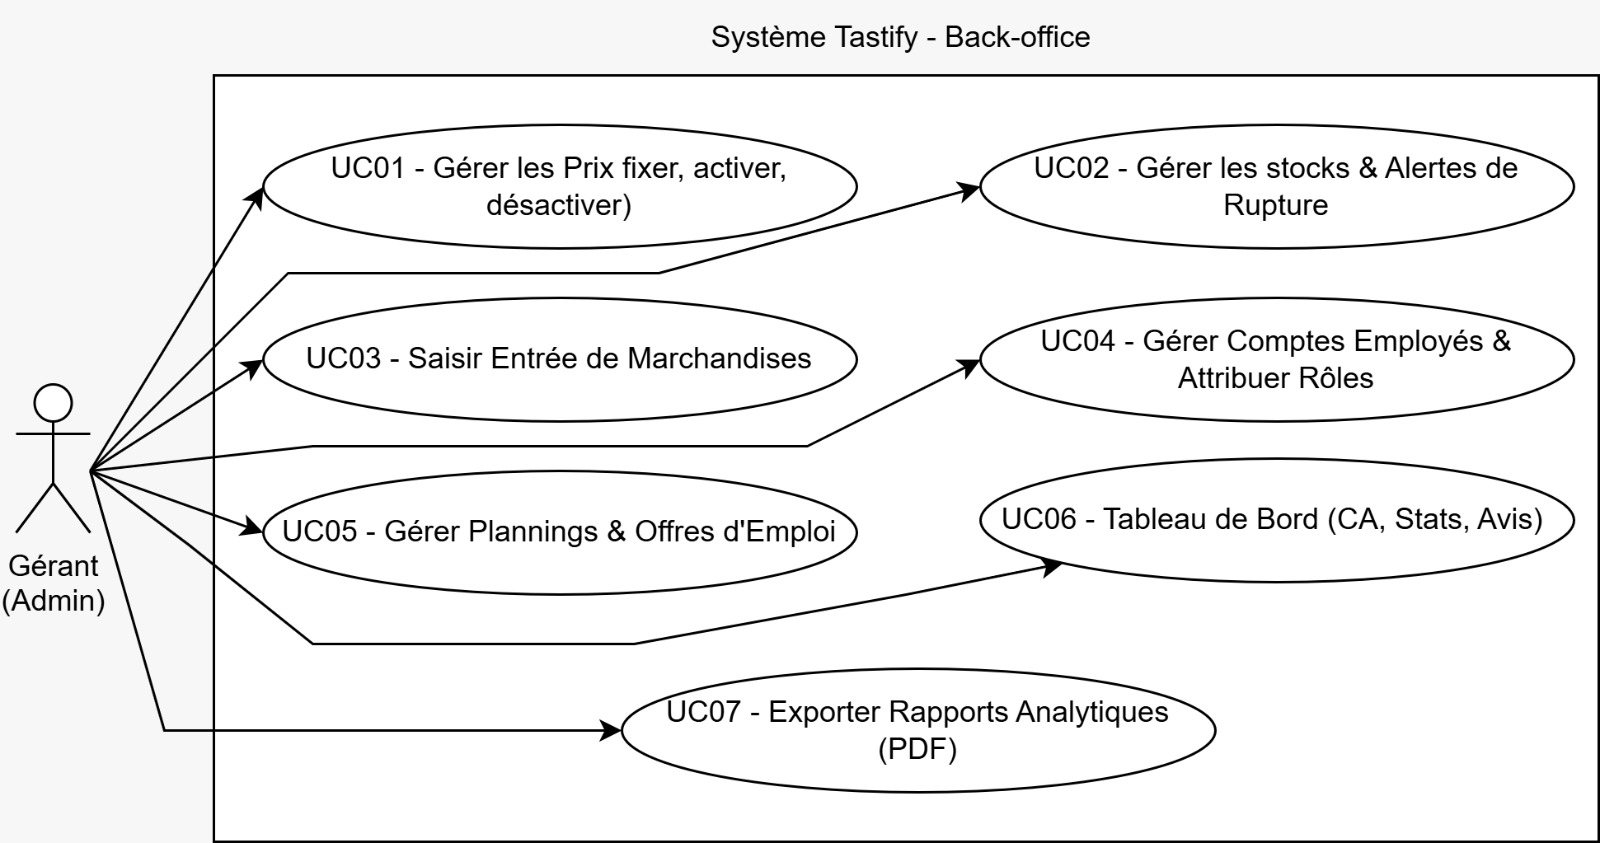
\includegraphics[width=\textwidth]{figure_08.jpeg}
\caption{Diagramme de cas d'utilisation du back-office gérant}
\label{fig:uc-admin}
\end{figure}

La figure~\ref{fig:uc-admin} regroupe les fonctions d'administration : menu, stock, employés, alertes, tableaux de bord et rapports.

\begin{figure}[H]
\centering
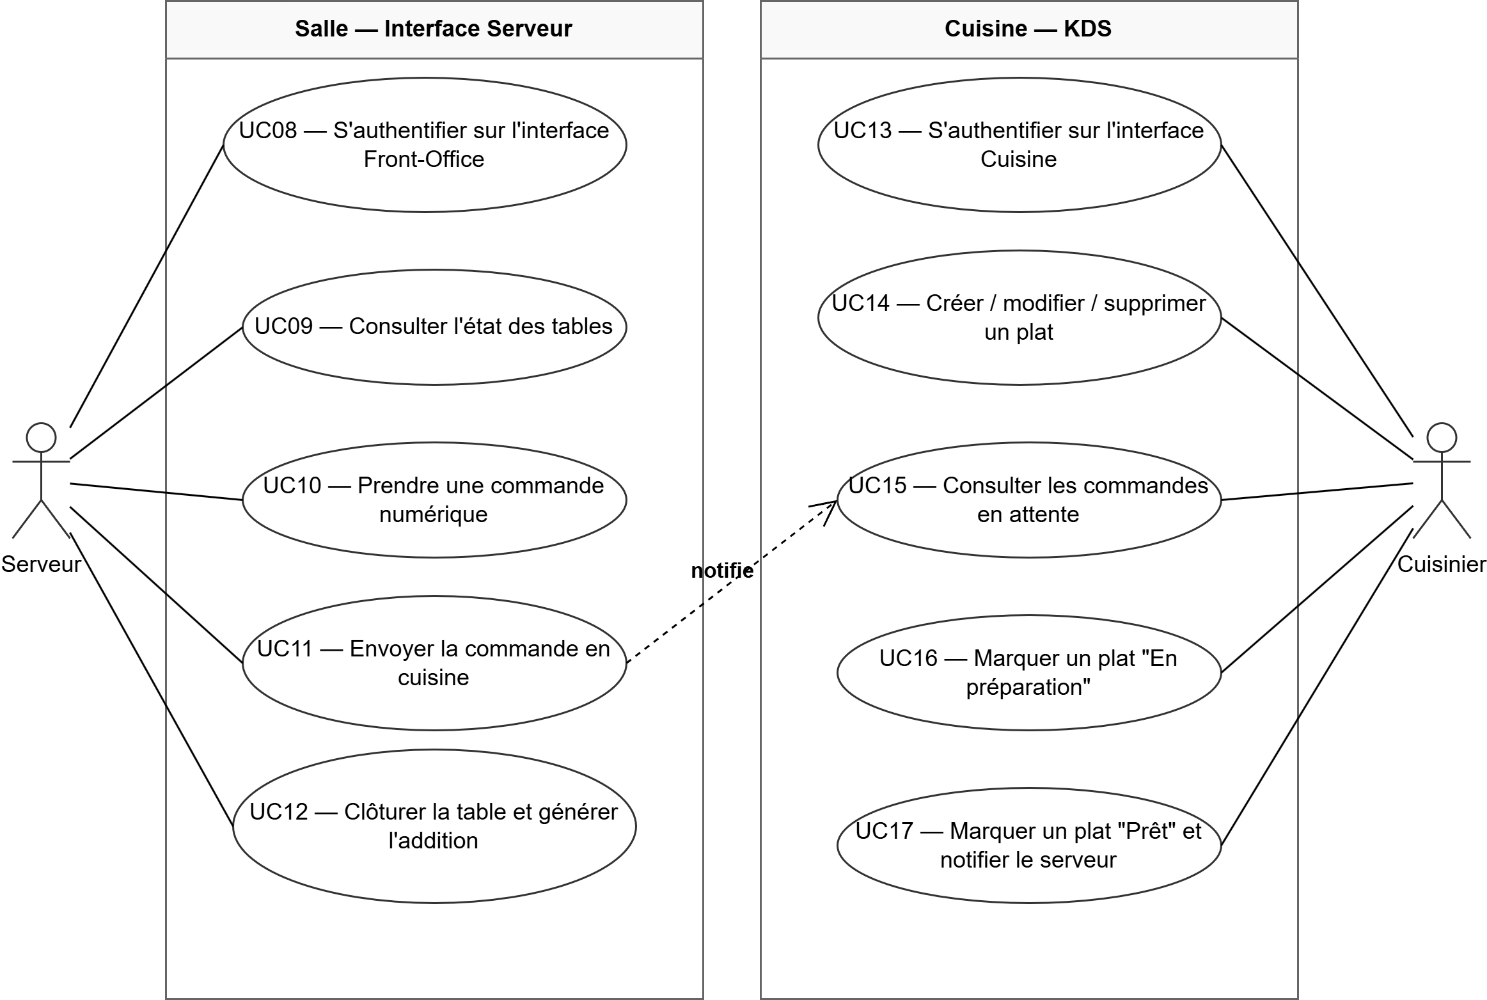
\includegraphics[width=\textwidth]{figure_05.png}
\caption{Diagramme de cas d'utilisation des modules salle et cuisine}
\label{fig:uc-salle-cuisine}
\end{figure}

La figure~\ref{fig:uc-salle-cuisine} montre le lien entre le serveur, la salle et le KDS. Elle explique le besoin de temps réel : la commande doit passer de l'interface serveur vers l'écran cuisine sans attente inutile.

\begin{figure}[H]
\centering
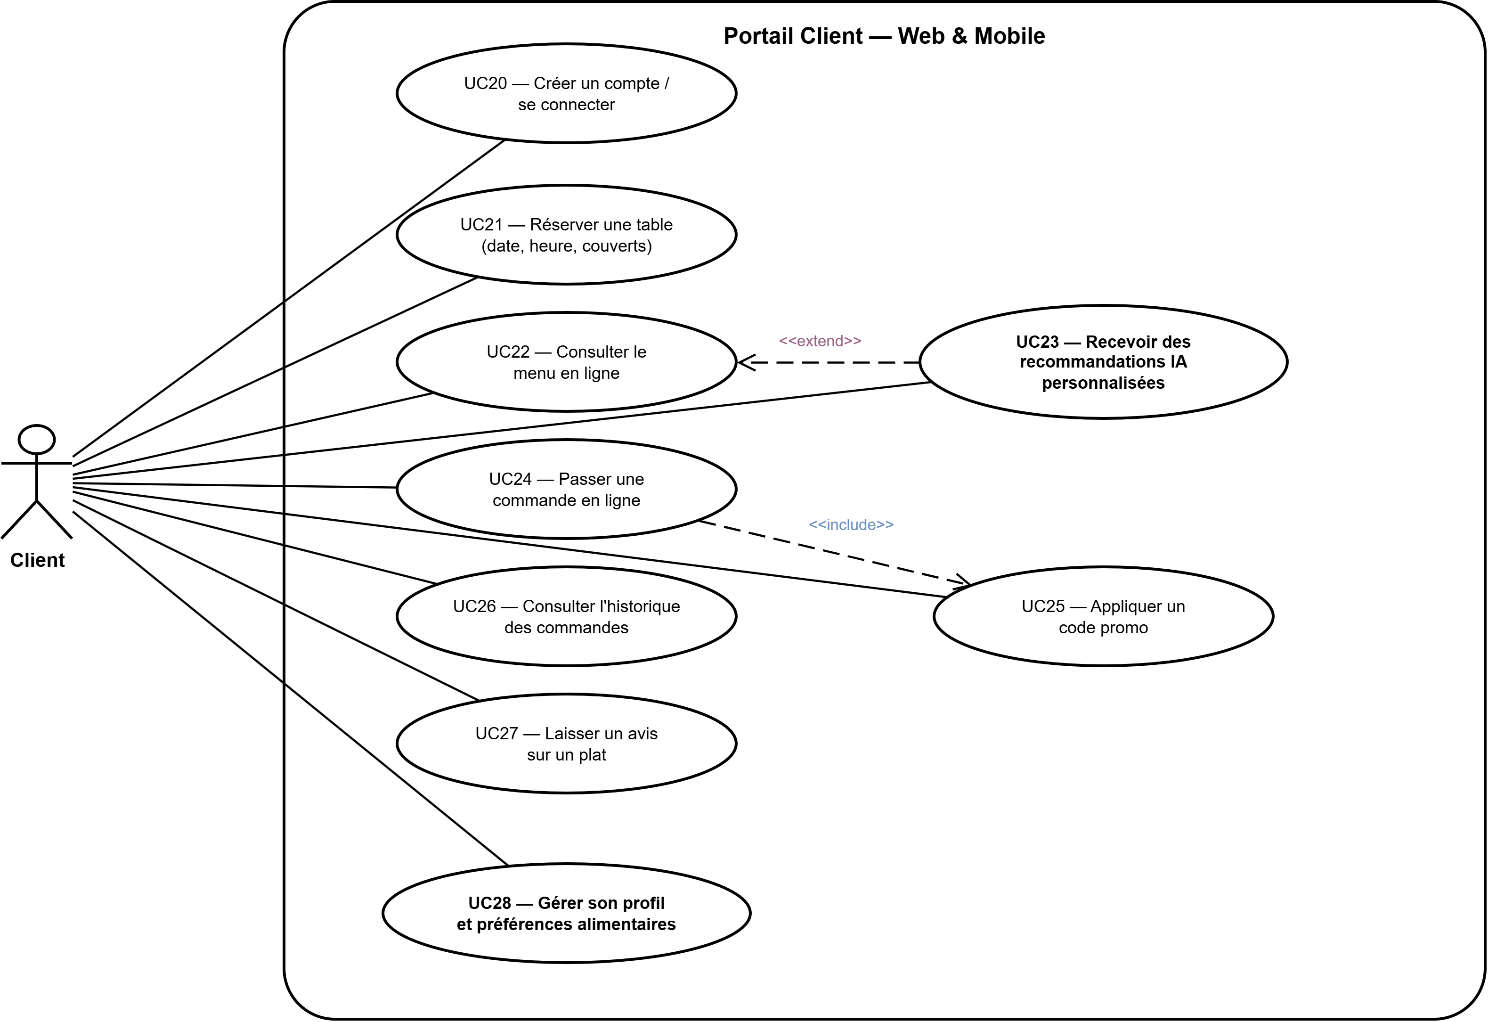
\includegraphics[width=0.98\textwidth]{figure_02.png}
\caption{Diagramme de cas d'utilisation du portail client}
\label{fig:uc-client}
\end{figure}

La figure~\ref{fig:uc-client} présente les fonctions disponibles côté client : consultation du menu, réservation, commande, paiement, fidélité et avis.

\section{Diagramme de classes}
Le diagramme de classes présente les entités majeures et leurs relations.

\clearpage
\begin{landscape}
\begin{figure}[p]
\centering
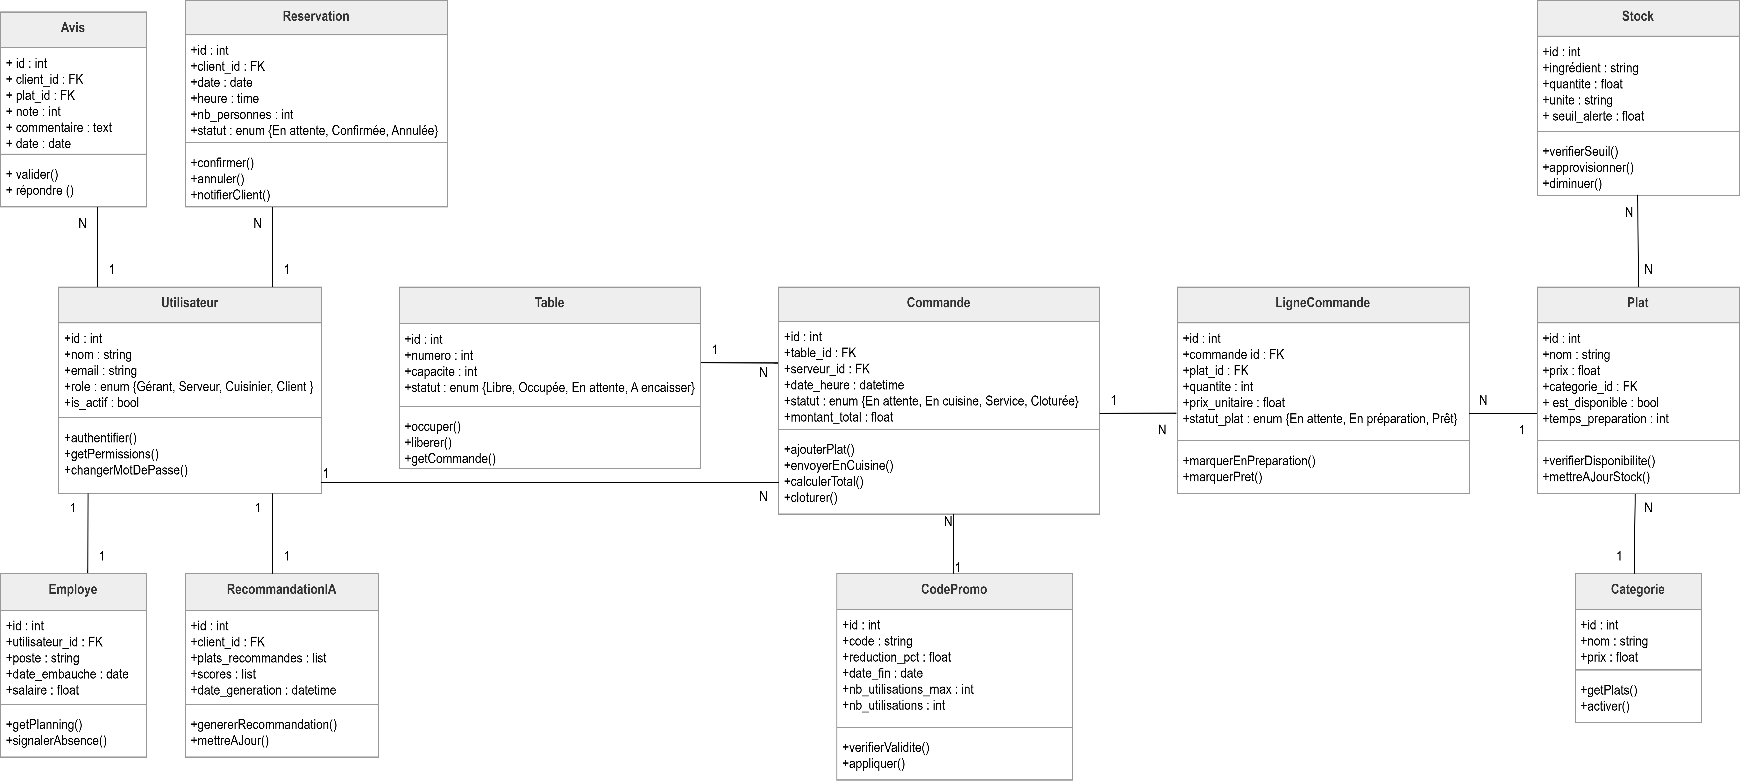
\includegraphics[width=0.95\linewidth,height=0.82\textheight,keepaspectratio]{figure_03.png}
\caption{Diagramme de classes de Tastify}
\label{fig:classes}
\end{figure}
\end{landscape}
\clearpage

La figure~\ref{fig:classes} correspond aux domaines présents dans l'application : utilisateurs, plats, tables, commandes, réservations, paiements, avis et stock. Certaines entités détaillées dans le code ne sont pas toutes visibles sur le schéma structurel initial ; elles sont donc précisées dans le modèle logique ci-dessous.

\section{Diagrammes de séquence}
Afin d'illustrer la dynamique des échanges et le comportement du système lors de scénarios clés, trois diagrammes de séquence sont introduits ci-dessous.

\subsection{Authentification staff}
Le processus d'authentification sécurisé pour les membres du personnel repose sur des jetons JWT. Le serveur, le cuisinier ou le gérant fournit ses identifiants qui sont validés par l'API backend avant d'émettre les clés de session, comme le montre la figure~\ref{fig:seq-auth}.

\begin{figure}[H]
\centering
\resizebox{\textwidth}{!}{%
\begin{tikzpicture}[>=stealth]
  \colorlet{pboxfill}{amber!10}
  \colorlet{pboxdraw}{amber!80!black}
  \colorlet{actfill}{gray!20}
  \colorlet{actdraw}{gray!60}
  \colorlet{msgcolor}{blue!60!black}
  \tikzset{
    participant/.style={draw=pboxdraw, fill=pboxfill, rounded corners=2pt, minimum width=2.8cm, minimum height=0.65cm, align=center, font=\bfseries\small},
    activation/.style={draw=actdraw, fill=actfill},
    msg/.style={thick, msgcolor},
    ret/.style={thick, dashed, gray!80!black},
    note/.style={midway, above, fill=white, inner sep=1.5pt, font=\scriptsize}
  }

  \foreach \x/\name in {0/Personnel,4.3/Interface Staff,8.6/API Backend,12.9/Base données} {
    \node[participant] at (\x,0) {\name};
    \draw[dashed, thick, gray!55] (\x,-0.45) -- (\x,-6.35);
  }

  \draw[activation] (-0.09,-0.8) rectangle (0.09,-1.25);
  \draw[activation] (4.21,-1.05) rectangle (4.39,-2.55);
  \draw[activation] (8.51,-2.25) rectangle (8.69,-5.2);
  \draw[activation] (12.81,-3.25) rectangle (12.99,-4.25);
  \draw[activation] (4.21,-4.75) rectangle (4.39,-5.8);

  \draw[->, msg] (0.12,-1.05) -- node[note, align=center] {1. Identifiants\\nom + code} (4.18,-1.05);
  \draw[->, msg] (4.42,-2.05) -- node[note] {2. POST \code{/api/token/}} (8.48,-2.05);
  \draw[->, msg] (8.72,-3.05) -- node[note] {3. Vérifier rôle} (12.78,-3.05);
  \draw[<-, ret] (8.72,-4.05) -- node[note] {4. Profil validé} (12.78,-4.05);
  \draw[<-, ret] (4.42,-5.0) -- node[note, align=center] {5. Token\\+ cookie} (8.48,-5.0);
  \draw[<-, msg] (0.12,-5.65) -- node[note] {6. Accès dashboard} (4.18,-5.65);
\end{tikzpicture}
}
\caption{Diagramme de séquence de l'authentification staff}
\label{fig:seq-auth}
\end{figure}

La figure~\ref{fig:seq-auth} détaille la séparation entre la saisie côté interface, la validation par l'API et la vérification du rôle en base de données avant l'accès au tableau de bord.

\subsection{Prise de commande et envoi vers le KDS}
Ce scénario décrit le flux de traitement en temps réel depuis la prise de commande par le serveur en salle jusqu'à sa diffusion instantanée vers l'écran de cuisine KDS grâce au protocole WebSocket géré par Redis, comme le montre la figure~\ref{fig:seq-commande-kds}.

\begin{figure}[H]
\centering
\resizebox{\textwidth}{!}{%
\begin{tikzpicture}[>=stealth]
  \colorlet{pboxfill}{amber!10}
  \colorlet{pboxdraw}{amber!80!black}
  \colorlet{actfill}{gray!20}
  \colorlet{actdraw}{gray!60}
  \colorlet{msgcolor}{blue!60!black}
  \tikzset{
    participant/.style={draw=pboxdraw, fill=pboxfill, rounded corners=2pt, minimum width=2.65cm, minimum height=0.65cm, align=center, font=\bfseries\small},
    activation/.style={draw=actdraw, fill=actfill},
    msg/.style={thick, msgcolor},
    ret/.style={thick, dashed, gray!80!black},
    note/.style={midway, above, fill=white, inner sep=1.5pt, font=\scriptsize}
  }

  \foreach \x/\name in {0/Serveur,3.65/Interface,7.3/API Backend,10.95/Serveur WS,14.6/KDS Cuisine} {
    \node[participant] at (\x,0) {\name};
    \draw[dashed, thick, gray!55] (\x,-0.45) -- (\x,-7.25);
  }

  \draw[activation] (-0.09,-0.75) rectangle (0.09,-1.2);
  \draw[activation] (3.56,-1.0) rectangle (3.74,-4.2);
  \draw[activation] (7.21,-1.95) rectangle (7.39,-5.2);
  \draw[activation] (10.86,-4.85) rectangle (11.04,-6.2);
  \draw[activation] (14.51,-5.85) rectangle (14.69,-7.0);

  \draw[->, msg] (0.12,-1.0) -- node[note] {1. Table et plats} (3.53,-1.0);
  \draw[->, msg] (3.77,-1.95) -- node[note] {2. Créer commande} (7.18,-1.95);
  \draw[->, msg] (7.42,-2.85) -- ++(0.75,0) -- ++(0,-0.55) -- node[right, align=left, fill=white, inner sep=1.5pt, font=\scriptsize, pos=0.55] {3. Sauvegarde\\en base} (7.42,-3.4);
  \draw[<-, ret] (3.77,-4.0) -- node[note] {4. Commande créée} (7.18,-4.0);
  \draw[->, msg] (7.42,-4.95) -- node[note] {5. Notification staff} (10.83,-4.95);
  \draw[->, msg] (11.07,-5.95) -- node[note] {6. Broadcast WS} (14.48,-5.95);
  \draw[->, msg] (14.6,-6.75) -- ++(0.75,0) -- ++(0,-0.35) -- node[right, align=left, fill=white, inner sep=1.5pt, font=\scriptsize, pos=0.45] {7. Affichage\\temps réel} (14.6,-7.1);
\end{tikzpicture}
}
\caption{Diagramme de séquence de la prise de commande et envoi au KDS}
\label{fig:seq-commande-kds}
\end{figure}

La figure~\ref{fig:seq-commande-kds} met en évidence le passage de la commande depuis l'interface staff vers l'API, puis la notification WebSocket qui permet au KDS cuisine de se mettre à jour en temps réel.

\subsection{Création d'un avis client et analyse de sentiment}
Le client soumet son commentaire et sa note depuis le portail public. Le backend enregistre l'avis et délègue en tâche d'arrière-plan Celery l'appel à l'API de traitement de langage naturel de Hugging Face pour classer le sentiment, comme le montre la figure~\ref{fig:seq-avis-sentiment}.

\begin{figure}[H]
\centering
\resizebox{\textwidth}{!}{%
\begin{tikzpicture}[>=stealth]
  \colorlet{pboxfill}{amber!10}
  \colorlet{pboxdraw}{amber!80!black}
  \colorlet{actfill}{gray!20}
  \colorlet{actdraw}{gray!60}
  \colorlet{msgcolor}{blue!60!black}
  \tikzset{
    participant/.style={draw=pboxdraw, fill=pboxfill, rounded corners=2pt, minimum width=2.65cm, minimum height=0.65cm, align=center, font=\bfseries\small},
    activation/.style={draw=actdraw, fill=actfill},
    msg/.style={thick, msgcolor},
    ret/.style={thick, dashed, gray!80!black},
    note/.style={midway, above, fill=white, inner sep=1.5pt, font=\scriptsize}
  }

  \foreach \x/\name in {0/Client,3.65/Portail Client,7.3/API Backend,10.95/Celery,14.6/Analyse} {
    \node[participant] at (\x,0) {\name};
    \draw[dashed, thick, gray!55] (\x,-0.45) -- (\x,-8.3);
  }

  \draw[activation] (-0.09,-0.75) rectangle (0.09,-1.2);
  \draw[activation] (3.56,-1.0) rectangle (3.74,-4.0);
  \draw[activation] (7.21,-1.9) rectangle (7.39,-4.45);
  \draw[activation] (10.86,-2.85) rectangle (11.04,-7.35);
  \draw[activation] (14.51,-4.75) rectangle (14.69,-6.0);
  \draw[activation] (7.21,-6.85) rectangle (7.39,-8.05);

  \draw[->, msg] (0.12,-1.0) -- node[note] {1. Avis et note} (3.53,-1.0);
  \draw[->, msg] (3.77,-1.95) -- node[note] {2. Créer avis} (7.18,-1.95);
  \draw[->, msg] (7.42,-2.95) -- node[note] {3. Tâche Celery} (10.83,-2.95);
  \draw[<-, ret] (3.77,-3.85) -- node[note] {4. Avis créé} (7.18,-3.85);
  \draw[->, msg] (11.07,-4.95) -- node[note] {5. Inférence IA} (14.48,-4.95);
  \draw[<-, ret] (11.07,-5.85) -- node[note] {6. Label + score} (14.48,-5.85);
  \draw[->, msg] (10.83,-6.9) -- node[note] {7. Sauvegarder sentiment} (7.42,-6.9);
  \draw[->, msg] (7.42,-7.65) -- ++(0.75,0) -- ++(0,-0.45) -- node[right, align=left, fill=white, inner sep=1.5pt, font=\scriptsize, pos=0.55] {8. Mise à jour\\stats gérant} (7.42,-8.1);
\end{tikzpicture}
}
\caption{Diagramme de séquence de la création d'un avis et analyse de sentiment}
\label{fig:seq-avis-sentiment}
\end{figure}

La figure~\ref{fig:seq-avis-sentiment} montre que la création de l'avis reste rapide pour le client, tandis que l'analyse est exécutée ensuite par Celery puis sauvegardée pour alimenter les statistiques.

\section{Modèle logique de données}
Le modèle logique de données est construit à partir des modèles Django de la codebase. Le tableau~\ref{tab:mld-resume} ne liste pas toutes les colonnes techniques. Il résume les tables structurantes et leurs relations.

\begin{longtable}{p{3.2cm}p{4.2cm}p{6.2cm}}
\caption{Synthèse du modèle logique de données}
\label{tab:mld-resume}\\
\toprule
\textbf{Table / entité} & \textbf{Relations principales} & \textbf{Rôle} \\
\midrule
\endfirsthead
\toprule
\textbf{Table / entité} & \textbf{Relations principales} & \textbf{Rôle} \\
\midrule
\endhead
\code{Utilisateur} & Rôle applicatif. & Compte de connexion et séparation gérant, serveur, cuisinier, client. \\
\code{Categorie}, \code{Plat} & Catégorie 1..N plats. & Structure de la carte, prix, disponibilité, image et temps de préparation. \\
\code{Ingredient}, \code{PlatIngredient} & Relation N..M entre plats et ingrédients. & Recettes et quantités requises pour relier menu et stock. \\
\code{Table}, \code{PlanText} & Table liée aux commandes et réservations. & Plan de salle, capacité, position et statut opérationnel. \\
\code{Commande}, \code{CommandeLigne} & Commande 1..N lignes ; table, serveur ou client optionnels. & Prise de commande, suivi cuisine, prix figé et total. \\
\code{Reservation} & Client, table, date et créneau. & Réservation avec statut et contrôle de disponibilité. \\
\code{Paiement}, \code{PaiementItem} & Paiement lié à une commande ; contributions liées aux lignes. & Encaissement et partage possible de l'addition. \\
\code{Avis}, \code{Analyse}\\\code{Sentiment} & Avis 1..1 analyse ; avis lié à plat ou commande. & Commentaire client, note optionnelle, label et score de sentiment. \\
\code{LoyaltyProfile}, \code{Reward} & Profil 1..1 utilisateur ; transactions et récompenses. & Programme de fidélité. \\
\code{WeatherData} & Données datées. & Support aux indicateurs et prévisions simples. \\
\code{Restaurant}\\\code{Configuration} & Configuration unique. & Paramètres du restaurant, identité, devise et réglages de service. \\
\bottomrule
\end{longtable}

\section{Règles métier principales}
Les règles suivantes structurent le comportement attendu :

\begin{itemize}
  \item un utilisateur possède un rôle qui détermine les routes et les actions accessibles ;
  \item une commande peut être liée à une table, à un serveur et parfois à un client ;
  \item chaque ligne de commande conserve le prix unitaire du plat au moment de la commande ;
  \item les statuts de lignes pilotent le KDS : attente, préparation, prêt, servi ou annulé ;
  \item un paiement est toujours lié à une commande et peut comporter des contributions par ligne ;
  \item un avis appartient à un utilisateur et peut être lié à un plat ou à une commande ;
  \item une analyse de sentiment est associée à un seul avis ;
  \item le stock repose sur les ingrédients, les seuils d'alerte et les mouvements.
\end{itemize}

\section{Architecture fonctionnelle cible}
La conception sépare deux usages : une application staff pour les rôles internes et un portail client. Les deux utilisent le même backend API.

\begin{figure}[H]
\centering
\fbox{\begin{minipage}{0.94\textwidth}
\centering
\schemaNode{Application staff\\Gérant, serveur, cuisinier}
\schemaArrow
\schemaNode{Backend Django REST Framework\\API REST, permissions}
\schemaArrow
\schemaNode{MySQL\\Données métier}

\vspace{0.45cm}

\schemaNode{Portail client\\Menu, réservation, paiement}
\schemaArrow
\schemaNode{Redis\\WebSocket et broker}
\schemaArrow
\schemaNode{Celery + Hugging Face\\Tâches et sentiment}
\end{minipage}}
\caption{Architecture fonctionnelle générale de Tastify}
\label{fig:architecture-fonctionnelle}
\end{figure}

La figure~\ref{fig:architecture-fonctionnelle} résume le choix principal du projet : un backend commun expose les services, tandis que les interfaces restent séparées selon les usages.

\section*{Conclusion}
\addcontentsline{toc}{section}{Conclusion}
L'analyse des besoins fait apparaître un système multi-acteurs, organisé autour d'un backend commun et de deux interfaces web. Les diagrammes existants donnent une base UML, complétée par le modèle logique tiré du code. Le chapitre suivant détaille l'analyse de sentiment, utilisée pour traiter les retours clients.

\chapter{Analyse de sentiment et choix du modèle}
\label{chap:sentiment}

\section*{Introduction}
\addcontentsline{toc}{section}{Introduction}
L'analyse de sentiment est la partie d'intelligence applicative la plus visible dans Tastify. Elle ne remplace pas le jugement du gérant, mais elle transforme les avis textuels en indicateurs simples : sentiment positif, neutre ou négatif, score de confiance et modèle utilisé.

\section{Rôle de l'analyse de sentiment dans Tastify}
Dans Tastify, les avis clients donnent un retour direct sur l'expérience au restaurant. Un commentaire peut signaler un plat apprécié, un service lent, une attente trop longue, une mauvaise température ou une satisfaction générale. Sans traitement automatique, ces retours deviennent difficiles à suivre dès que leur nombre augmente.

L'analyse de sentiment joue donc deux rôles :

\begin{itemize}
  \item \textbf{opérationnel}, car elle aide le gérant à repérer rapidement les avis défavorables ;
  \item \textbf{analytique}, car elle alimente les statistiques de satisfaction affichées dans le tableau de bord.
\end{itemize}

L'implémentation couvre les statistiques de sentiment dans les indicateurs. Le résultat de l'analyse est donc exploité par l'application, il n'est pas seulement stocké.

\section{Données utilisées}
Le projet ne contient pas de jeu de données local destiné à entraîner un modèle propriétaire. Tastify utilise les avis saisis par les utilisateurs de l'application.

\begin{table}[H]
\centering
\caption{Données utilisées par le pipeline de sentiment}
\label{tab:donnees-sentiment}
\begin{tabularx}{\textwidth}{p{3.4cm}Y}
\toprule
\textbf{Champ} & \textbf{Utilisation} \\
\midrule
\pathcode{Avis.commentaire} & Texte libre analysé par le pipeline. C'est l'entrée principale du modèle. \\
\pathcode{Avis.note} & Note optionnelle entre 1 et 5. Elle est stockée, mais le code d'analyse actuel se base sur le commentaire. \\
\pathcode{Avis.lang_code} & Langue détectée simplement : \code{ar} si le texte contient des caractères arabes, \code{en} sinon. \\
\pathcode{AnalyseSentiment.label} & Résultat normalisé : \code{POSITIF}, \code{NEUTRE} ou \code{NEGATIF}. \\
\pathcode{AnalyseSentiment.score_brut} & Score de confiance renvoyé par Hugging Face ou par le fallback local. \\
\pathcode{AnalyseSentiment.modele_utilise} & Nom du modèle distant ou de la méthode locale réellement utilisée. \\
\bottomrule
\end{tabularx}
\end{table}

Le texte envoyé à Hugging Face est limité à 512 caractères dans la tâche Celery. Ce choix suffit pour des avis courts et évite d'envoyer des commentaires trop longs au modèle.

\section{Pipeline technique}
Le pipeline démarre lors de la création d'un avis dans le \code{AvisViewSet}. L'avis est enregistré rapidement, puis l'analyse est confiée à une tâche Celery.

\begin{figure}[H]
\centering
\fbox{\begin{minipage}{0.94\textwidth}
\centering
\schemaNode{Portail client\\saisie avis}
\schemaArrow
\schemaNode{API \code{/api/avis/}\\création}
\schemaArrow
\schemaNode{Tâche Celery\\analyse}

\vspace{0.45cm}

\schemaNode{Hugging Face\\modèle distant}
\schemaArrow
\schemaNode{Fallback local\\mots-clés}
\schemaArrow
\schemaNode{MySQL + Dashboard\\résultat et statistiques}
\end{minipage}}
\caption{Pipeline technique de l'analyse de sentiment}
\label{fig:pipeline-sentiment}
\end{figure}

La figure~\ref{fig:pipeline-sentiment} résume le flux : l'utilisateur soumet un avis, le backend l'enregistre, Celery lance l'analyse, puis le résultat est stocké et agrégé dans les statistiques.

\begin{figure}[H]
\centering
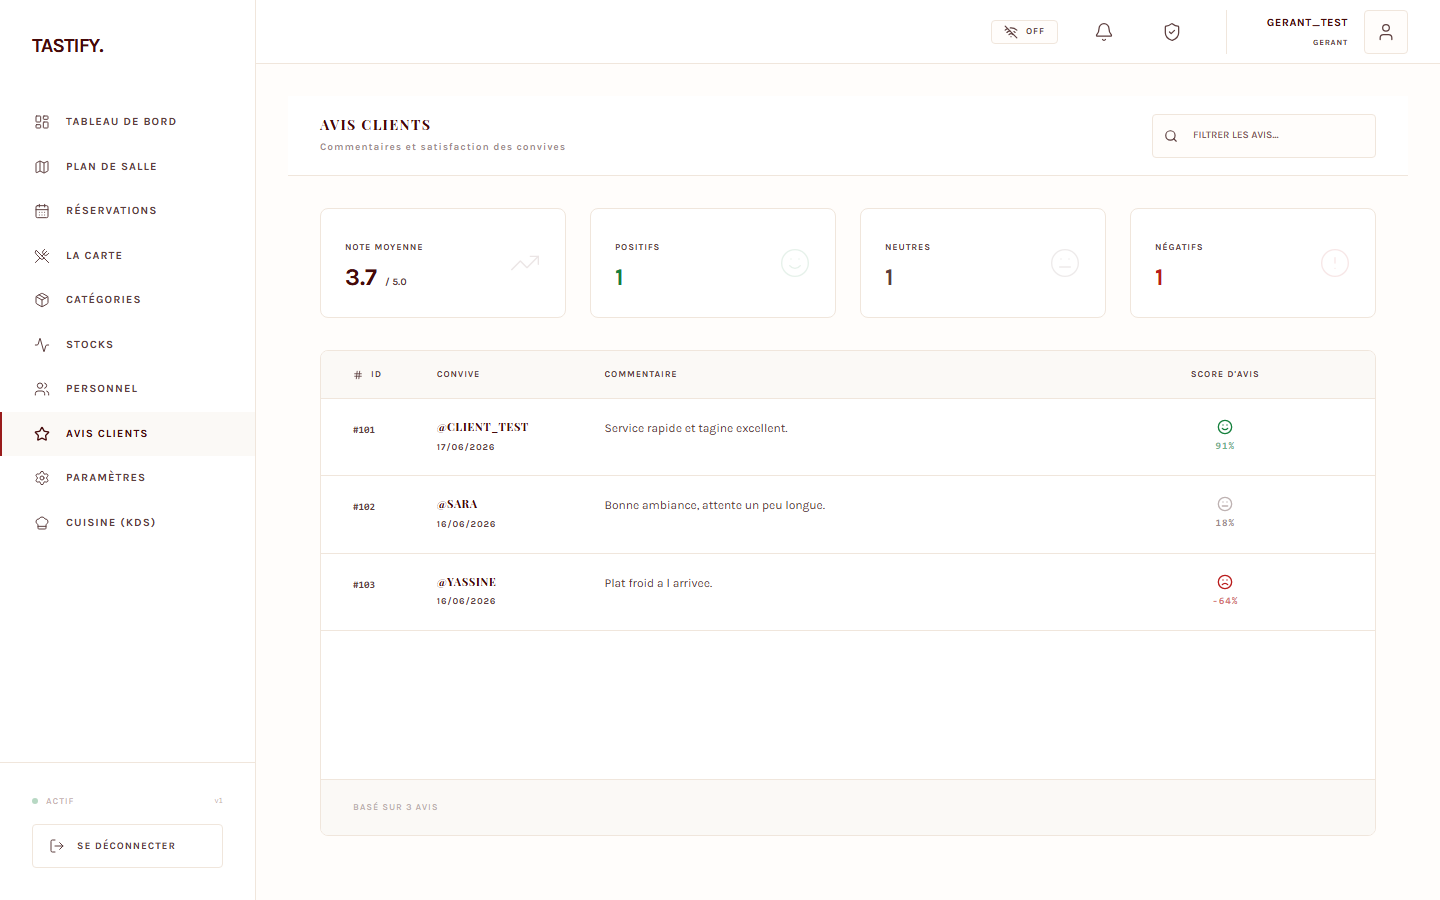
\includegraphics[width=0.95\textwidth]{capture_avis_sentiment.png}
\caption{Back-office : avis clients avec scores de sentiment}
\label{fig:capture-avis-sentiment}
\end{figure}

La figure~\ref{fig:capture-avis-sentiment} montre l'exploitation concrète du pipeline dans l'interface : chaque avis conserve son texte, sa note et un résultat de sentiment utilisable par le gérant pour prioriser les retours.

\section{Modèle réellement utilisé}
Le code du fichier \code{apps/avis/tasks.py} définit les modèles suivants :

\begin{itemize}
  \item \pathcode{nlptown/bert-base-multilingual-uncased-sentiment} pour les avis non arabes ;
  \item \pathcode{moussaKam/MARBERT-sentiment} pour les textes contenant des caractères arabes ;
  \item \pathcode{nlptown/bert-base-multilingual-uncased-sentiment} comme modèle de secours si le modèle arabe ne répond pas ;
  \item \pathcode{mots-cles-simple} comme secours local lorsque l'API Hugging Face n'est pas disponible ou lorsqu'aucun jeton n'est configuré.
\end{itemize}

Le modèle principal \pathcode{nlptown/bert-base-multilingual-uncased-sentiment} est un BERT multilingue affiné pour l'analyse de sentiment sur des avis produits en six langues, dont le français \cite{nlptown}. Il renvoie une prédiction sous forme d'étoiles de 1 à 5. Le code convertit ensuite cette sortie en trois classes : négatif, neutre ou positif. Ce choix correspond bien à un restaurant, car les commentaires clients ressemblent souvent à des avis courts sur un produit ou un service.

La base scientifique de ce type de modèle vient de BERT, qui apprend des représentations contextuelles bidirectionnelles et peut être adapté à des tâches de classification avec une couche de sortie \cite{bert}. Pour les textes arabes, le code utilise MARBERT, une famille de modèles conçus pour l'arabe et ses variantes dialectales \cite{marbert}.

\section{Conversion des sorties}
Les sorties du modèle ne sont pas exposées telles quelles au reste de l'application. Elles sont normalisées pour être lisibles dans le tableau de bord.

\begin{table}[H]
\centering
\caption{Normalisation des sorties de sentiment}
\label{tab:normalisation-sentiment}
\begin{tabularx}{\textwidth}{p{3.2cm}p{3.4cm}Y}
\toprule
\textbf{Sortie modèle} & \textbf{Label Tastify} & \textbf{Score métier} \\
\midrule
\code{5 stars}, \code{4 stars}, \code{POSITIVE}, \code{LABEL\_2} & \code{POSITIF} & $+15$, avis favorable. \\
\code{3 stars}, \code{NEUTRAL}, \code{LABEL\_1} & \code{NEUTRE} & $0$, signal sans polarité forte. \\
\code{1 star}, \code{2 stars}, \code{NEGATIVE}, \code{LABEL\_0} & \code{NEGATIF} & $-15$, avis défavorable à surveiller. \\
\bottomrule
\end{tabularx}
\end{table}

Cette conversion rend l'indicateur plus lisible pour le gérant, tout en gardant dans \code{score\_brut} la confiance renvoyée par le modèle.

\section{Comparaison avec des alternatives}
Le tableau~\ref{tab:comparaison-modeles} compare le modèle principal avec plusieurs alternatives possibles.

\begin{table}[p]
\centering
\scriptsize
\caption{Comparaison des approches de sentiment}
\label{tab:comparaison-modeles}
\begin{tabularx}{\textwidth}{p{3.2cm}p{2.5cm}YYY}
\toprule
\textbf{Approche} & \textbf{Statut dans Tastify} & \textbf{Forces} & \textbf{Limites} & \textbf{Pertinence} \\
\midrule
BERT multilingue NLP Town & Modèle principal & Supporte le français, l'anglais, l'espagnol, l'italien, l'allemand et le néerlandais ; entraîné sur des avis ; utilisable via API \cite{nlptown,hftextclassification}. & Moins spécialisé qu'un modèle français pur ; dépend d'un service externe si utilisé via API. & Très adapté aux avis courts de restaurant multilingues. \\
DistilCamemBERT sentiment & Alternative française & Spécialisé français ; modèle plus léger ; résultats documentés sur Amazon Reviews et Allociné \cite{distilcamembert,camembert}. & Ne couvre pas naturellement l'arabe ou l'anglais ; demande un routage par langue. & Bon choix si le périmètre devient surtout francophone. \\
XLM-R / XLM-T & Alternative multilingue & Bonne base de transfert multilingue ; XLM-R est conçu pour de nombreux langages \cite{xlmroberta}; XLM-T vise les textes sociaux multilingues \cite{xlmt}. & Demande un choix de modèle fine-tuné et des validations supplémentaires. & Intéressant pour une version multilingue plus avancée. \\
MARBERT sentiment & Modèle arabe utilisé & Appuyé sur la famille MARBERT, adaptée aux variétés arabes et au texte social \cite{marbert}. & Spécifique aux textes arabes ; ne remplace pas le modèle multilingue pour le français. & Adapté aux avis en arabe ou en dialecte marocain. \\
Mots-clés / TF-IDF local & Fallback partiel & Fonctionne hors ligne, transparent et peu coûteux ; le fallback actuel par mots-clés est déjà implémenté. & Faible face à l'ironie, aux négations et au vocabulaire varié ; TF-IDF n'est pas implémenté dans le dépôt. & Utile comme secours, mais insuffisant comme moteur principal. \\
\bottomrule
\end{tabularx}
\end{table}

\section{Justification du choix}
Le choix du modèle \pathcode{nlptown/bert-base-multilingual-uncased-sentiment} est défendable pour quatre raisons :

\begin{enumerate}
  \item \textbf{Proximité avec le domaine des avis.} Le modèle est affiné sur des avis, ce qui se rapproche des commentaires laissés sur des plats ou sur un restaurant.
  \item \textbf{Support du français.} La fiche du modèle indique un entraînement incluant le français, ce qui correspond au contexte du rapport et aux interfaces francophones.
  \item \textbf{Intégration rapide.} L'API Hugging Face permet de lancer l'inférence sans embarquer un modèle lourd dans le backend.
  \item \textbf{Continuité du service.} Le fallback local permet de produire un résultat même sans jeton Hugging Face ou en cas d'erreur réseau.
\end{enumerate}

Ce choix est cohérent avec le périmètre PFA et couvre les avis multilingues attendus dans Tastify. Pour une version de production, l'étape suivante serait de mesurer la qualité du modèle sur des avis du restaurant, constituer un petit jeu de validation local, puis comparer les scores entre le modèle multilingue, un modèle français spécialisé et un modèle arabe.

\section{Limites de la fonctionnalité}
Les limites suivantes sont identifiées :

\begin{itemize}
  \item la détection de langue reste simple : elle détecte l'arabe par présence de caractères arabes et classe le reste comme \code{en} ;
  \item le fallback local repose sur des listes de mots positifs et négatifs, pas sur un modèle statistique entraîné ;
  \item le projet ne fournit pas de métriques d'évaluation sur un corpus d'avis Tastify ;
  \item la note de 1 à 5 n'est pas combinée avec le commentaire pour améliorer la prédiction ;
  \item l'utilisation de Hugging Face suppose une configuration correcte du jeton \code{HUGGINGFACE\_API\_TOKEN}.
\end{itemize}

\section*{Conclusion}
\addcontentsline{toc}{section}{Conclusion}
L'analyse de sentiment de Tastify est intégrée au flux métier : elle tourne en arrière-plan, stocke son résultat et alimente les tableaux de bord. Le modèle principal correspond au contexte des avis clients, et une évaluation locale pourra renforcer encore sa précision dans une version de production.

\chapter{Architecture technique et réalisation}
\label{chap:realisation}

\section*{Introduction}
\addcontentsline{toc}{section}{Introduction}
Ce chapitre décrit la réalisation de Tastify. Il présente la stack technique, l'organisation du backend, les deux applications React, la sécurité, le temps réel, les modules métier, les interfaces et le déploiement.

\section{Stack technique}
Le projet utilise une architecture web découplée. Le backend expose des API REST et un canal WebSocket ; les frontends consomment ces services depuis deux applications React.

\begin{table}[H]
\centering
\caption{Stack technique confirmée}
\label{tab:stack}
\begin{tabularx}{\textwidth}{p{3.3cm}p{3.8cm}Y}
\toprule
\textbf{Couche} & \textbf{Technologies} & \textbf{Rôle} \\
\midrule
Backend & Python, Django, Django REST Framework & API REST, modèles, permissions, logique métier et documentation OpenAPI \cite{django,drf}. \\
Serveur ASGI & Daphne, Django Channels & Exécution asynchrone et WebSocket pour les événements staff \cite{channels}. \\
Base de données & MySQL & Persistance relationnelle des données métier \cite{mysql}. \\
Cache et messages & Redis & Channel layer WebSocket et broker Celery \cite{redis}. \\
Tâches asynchrones & Celery, Celery Beat & Analyse de sentiment, traitements de stock, orchestration et tâches planifiées \cite{celery}. \\
Frontends & React, Vite, TypeScript, Tailwind CSS & Applications SPA staff et client \cite{react,vite,tailwind}. \\
Tests & pytest, Vitest, Playwright & Validation backend, tests unitaires frontend et scénarios end-to-end. \\
Déploiement & Docker Compose & Orchestration des services locaux et préparation au déploiement \cite{docker}. \\
\bottomrule
\end{tabularx}
\end{table}

\section{Architecture globale}
La figure~\ref{fig:architecture-technique} présente l'organisation technique de la solution.

\begin{figure}[H]
\centering
\fbox{\begin{minipage}{0.94\textwidth}
\centering
\schemaNode{Back-office React\\port 3000}
\schemaArrow
\schemaNode{Backend Django ASGI\\REST + WebSocket\\port 8000}
\schemaArrow
\schemaNode{MySQL 8\\volume persistant}

\vspace{0.45cm}

\schemaNode{Portail client React\\port 3003}
\schemaArrow
\schemaNode{Redis 7\\WebSocket + broker}
\schemaArrow
\schemaNode{Celery worker / beat\\tâches de fond}
\end{minipage}}
\caption{Architecture technique de Tastify}
\label{fig:architecture-technique}
\end{figure}

Cette architecture sépare les responsabilités. Le backend concentre la logique métier. Les deux frontends restent centrés sur leurs usages : gestion interne pour le staff, expérience client pour le portail public.

\section{Organisation du backend}
Le backend est découpé en applications Django spécialisées. Ce choix rend chaque domaine plus lisible et simplifie les tests.

\begin{longtable}{p{3.5cm}p{10cm}}
\caption{Modules backend réalisés}
\label{tab:modules-backend}\\
\toprule
\textbf{Module} & \textbf{Responsabilité} \\
\midrule
\endfirsthead
\toprule
\textbf{Module} & \textbf{Responsabilité} \\
\midrule
\endhead
\code{users} & Utilisateur personnalisé, rôles, authentification JWT, refresh cookies et réinitialisation de mot de passe. \\
\code{menu} & Catégories, plats, disponibilité, images, liens avec les ingrédients et recommandations simples. \\
\code{tables} & Tables, capacités, positions, statuts et textes de plan. \\
\code{commandes} & Commandes, lignes, prix figés, statuts cuisine, signaux et orchestration KDS. \\
\code{stock} & Ingrédients, recettes, mouvements, seuils d'alerte et services d'approvisionnement. \\
\code{hr} & Employés, shifts, offres d'emploi et candidatures. \\
\code{reservations} & Réservations, disponibilité, conflits de créneaux, statuts et notifications. \\
\code{paiements} & Paiements, contributions par ligne, tokens de paiement et réconciliation commande-paiement. \\
\code{avis} & Avis clients, tâche d'analyse de sentiment et stockage du résultat. \\
\code{analytics} & Tableau de bord, revenus, plats populaires, statistiques de sentiment et données météo. \\
\code{loyalty} & Profils, transactions, points et récompenses. \\
\code{configuration} & Identité du restaurant, devise, couleurs et paramètres de service. \\
\bottomrule
\end{longtable}

\section{Authentification et sécurité}
L'authentification repose sur \code{djangorestframework-simplejwt}. Le backend émet un access token de courte durée et un refresh token stocké dans un cookie HttpOnly \cite{simplejwt}. Le projet intègre aussi une séparation staff/client pour éviter qu'une session ouverte sur un portail écrase l'autre.

\begin{figure}[H]
\centering
\fbox{\begin{minipage}{0.94\textwidth}
\centering
\schemaNode{Utilisateur\\identifiants}
\schemaArrow
\schemaNode{Frontend\\staff ou client}
\schemaArrow
\schemaNode{API auth Django\\vérification}
\schemaArrow
\schemaNode{Base utilisateur\\rôle}

\vspace{0.35cm}

\small Réponse : access token court + refresh token en cookie HttpOnly. Le refresh renouvelle l'accès sans exposer le jeton long côté JavaScript.
\end{minipage}}
\caption{Séquence simplifiée d'authentification JWT}
\label{fig:auth-jwt}
\end{figure}

Les accès sensibles sont protégés par les permissions DRF et par les gardes de rôles côté frontend. Le gérant accède aux écrans d'administration, le serveur aux fonctions de salle, le cuisinier au KDS, et le client au portail public et à son espace personnel.

\section{Temps réel et Kitchen Display System}
Le temps réel repose sur Django Channels et Redis. Le canal WebSocket \code{/ws/staff/} accepte seulement les rôles internes : gérant, serveur et cuisinier. Les événements staff mettent à jour les écrans sans recharger toute la page.

\begin{figure}[H]
\centering
\fbox{\begin{minipage}{0.94\textwidth}
\centering
\schemaNode{Serveur\\prise de commande}
\schemaArrow
\schemaNode{API commandes\\validation}
\schemaArrow
\schemaNode{MySQL\\commande}
\schemaArrow
\schemaNode{Redis\\staff group}

\vspace{0.35cm}

\schemaNode{KDS cuisine\\affichage}
\schemaArrow
\schemaNode{Cuisinier\\statut plat}
\schemaArrow
\schemaNode{API commandes\\mise à jour}
\end{minipage}}
\caption{Flux temps réel entre prise de commande et KDS}
\label{fig:flux-kds}
\end{figure}

La figure~\ref{fig:flux-kds} montre le flux principal : le serveur crée la commande, le backend l'enregistre, puis publie un événement vers le groupe staff. Le cuisinier peut ensuite mettre à jour les statuts de préparation.

\section{Applications frontend}
L'architecture comprend deux applications React distinctes.

\begin{table}[H]
\centering
\caption{Applications frontend}
\label{tab:frontends}
\begin{tabularx}{\textwidth}{p{3.3cm}p{3cm}Y}
\toprule
\textbf{Application} & \textbf{Port local} & \textbf{Fonction} \\
\midrule
Back-office staff & 3000 & Tableau de bord, menu, catégories, salle, réservations, KDS, stocks, RH, avis et paramètres. \\
Portail client & 3003 & Accueil, menu, réservation, compte, inscription, connexion, paiement, contact, fidélité et mode hors ligne. \\
\bottomrule
\end{tabularx}
\end{table}

Les routes frontend confirment la séparation des usages. Dans le back-office, les routes sont protégées par rôle. Dans le portail client, certaines pages sont publiques et d'autres demandent une authentification.

\section{Paiement et fidélité}
Le module de paiement associe chaque paiement à une commande. Il peut aussi relier des contributions aux lignes de commande, ce qui permet de représenter un paiement global ou un partage de l'addition. Les méthodes présentes dans le modèle couvrent notamment les espèces, la carte et le QR.

Le module fidélité repose sur un profil lié à l'utilisateur, des transactions de points et des récompenses. Les paliers calculés à partir du solde de points ajoutent une logique de relation client sans alourdir l'usage principal.

\section{Stocks et prévision simple}
Le module stock relie les plats à leurs ingrédients grâce à une table de recette. Les mouvements de stock servent à suivre les entrées, les sorties et les ajustements. Les seuils d'alerte permettent d'identifier les ingrédients à surveiller.

Dans cette version, la partie approvisionnement et météo reste limitée à une estimation métier simple, utile pour anticiper certains besoins sans la confondre avec un modèle prédictif avancé entraîné localement.

\section{Moteur de recommandation de plats}
Tastify intègre un moteur de recommandation pour suggérer des plats aux clients sur le portail public. Le socle prévu pour l'évolution avancée repose sur une logique item-based calculable à partir des co-occurrences de commande.

L'algorithme, implémenté dans le module \pathcode{apps/menu/ml/recommender.py}, analyse l'historique de toutes les lignes de commande via la méthode \code{compute\_similarities}. Pour chaque paire de plats commandés ensemble dans une même transaction, un score de co-occurrence est incrémenté. Les résultats de cette matrice de similarité symétrique sont stockés dans le cache Redis pour des performances optimales lors de la navigation du client.

Sur la page d'accueil du portail client, les plats recommandés issus de l'action \code{top-recommendations} s'affichent sous la forme de suggestions, enrichies du premier avis positif du plat s'il existe. Cette action classe les plats par moyenne de \code{sentiment\_score} décroissante, puis par nombre d'avis analysés. Les plats ayant les retours les plus positifs apparaissent donc en premier dans la zone de recommandation.

\section{Interfaces réalisées}
Les captures suivantes proviennent de l'environnement local de démonstration Tastify. Elles sont intégrées dans le corps du rapport afin de montrer directement les modules livrés.

\begin{figure}[H]
\centering
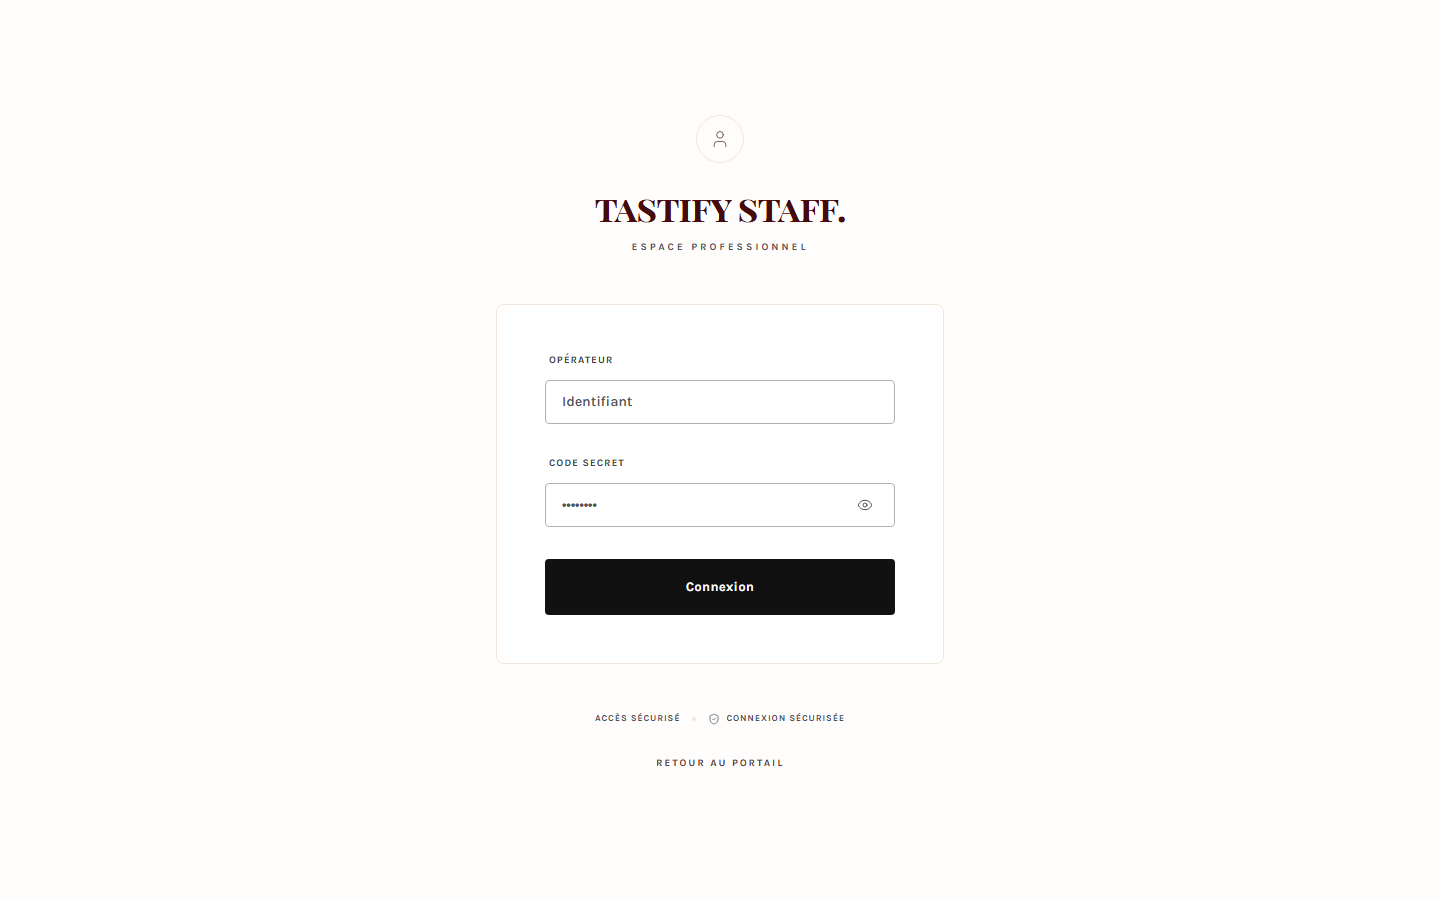
\includegraphics[width=0.95\textwidth]{capture_login_staff.png}
\caption{Connexion staff : accès sécurisé au back-office}
\label{fig:capture-login-staff}
\end{figure}

La figure~\ref{fig:capture-login-staff} illustre le point d'entrée réservé au personnel, avec une authentification séparée du portail client.

\begin{figure}[H]
\centering
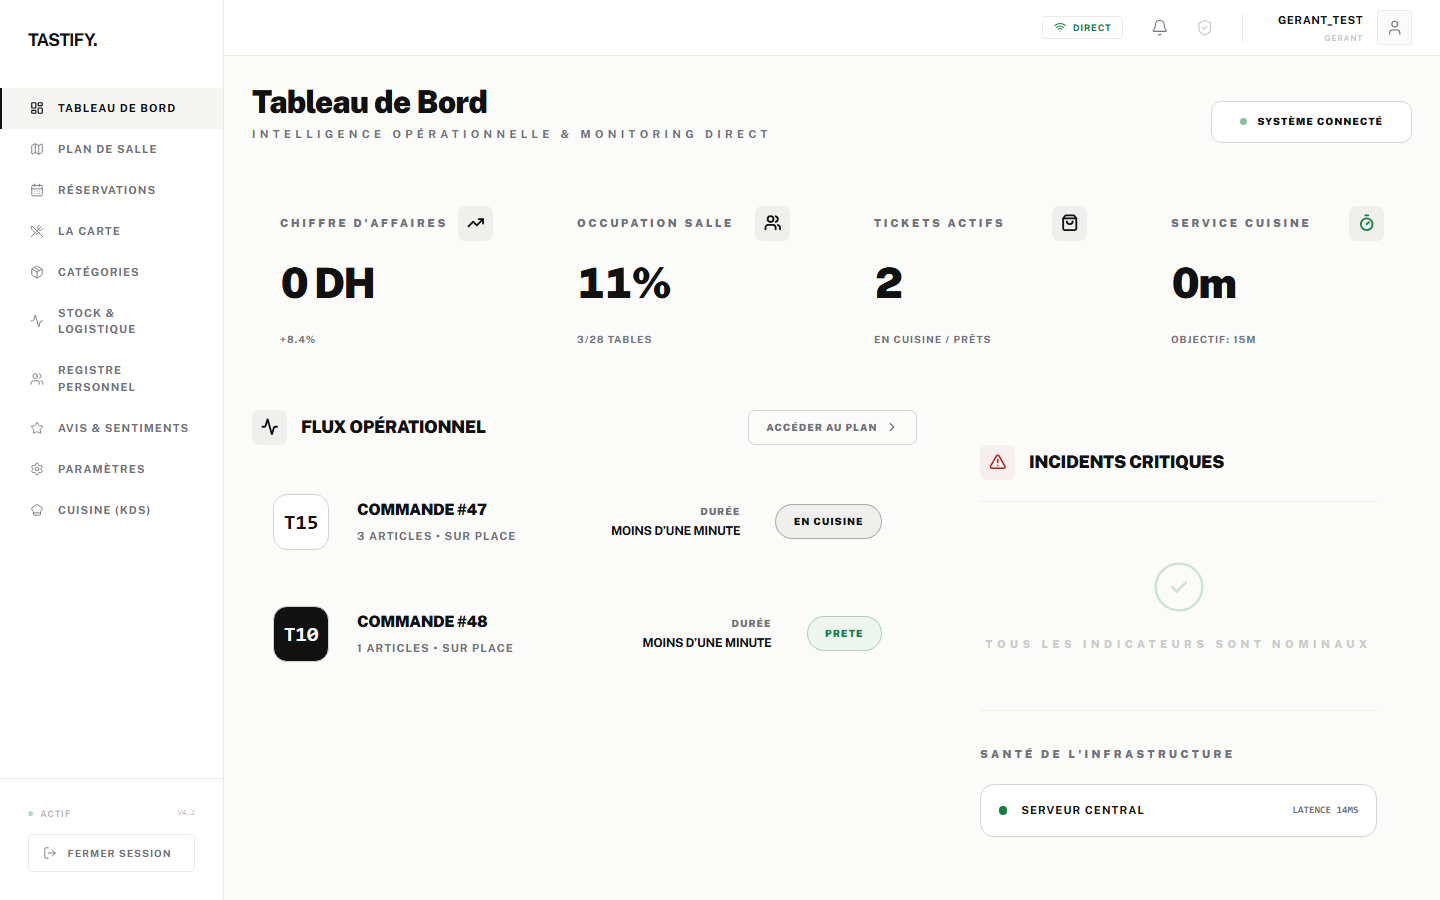
\includegraphics[width=0.95\textwidth]{capture_dashboard.png}
\caption{Tableau de bord gérant du back-office}
\label{fig:capture-dashboard}
\end{figure}

La figure~\ref{fig:capture-dashboard} présente la vue de pilotage du gérant, où les indicateurs métier sont regroupés pour faciliter le suivi quotidien.

\begin{figure}[H]
\centering
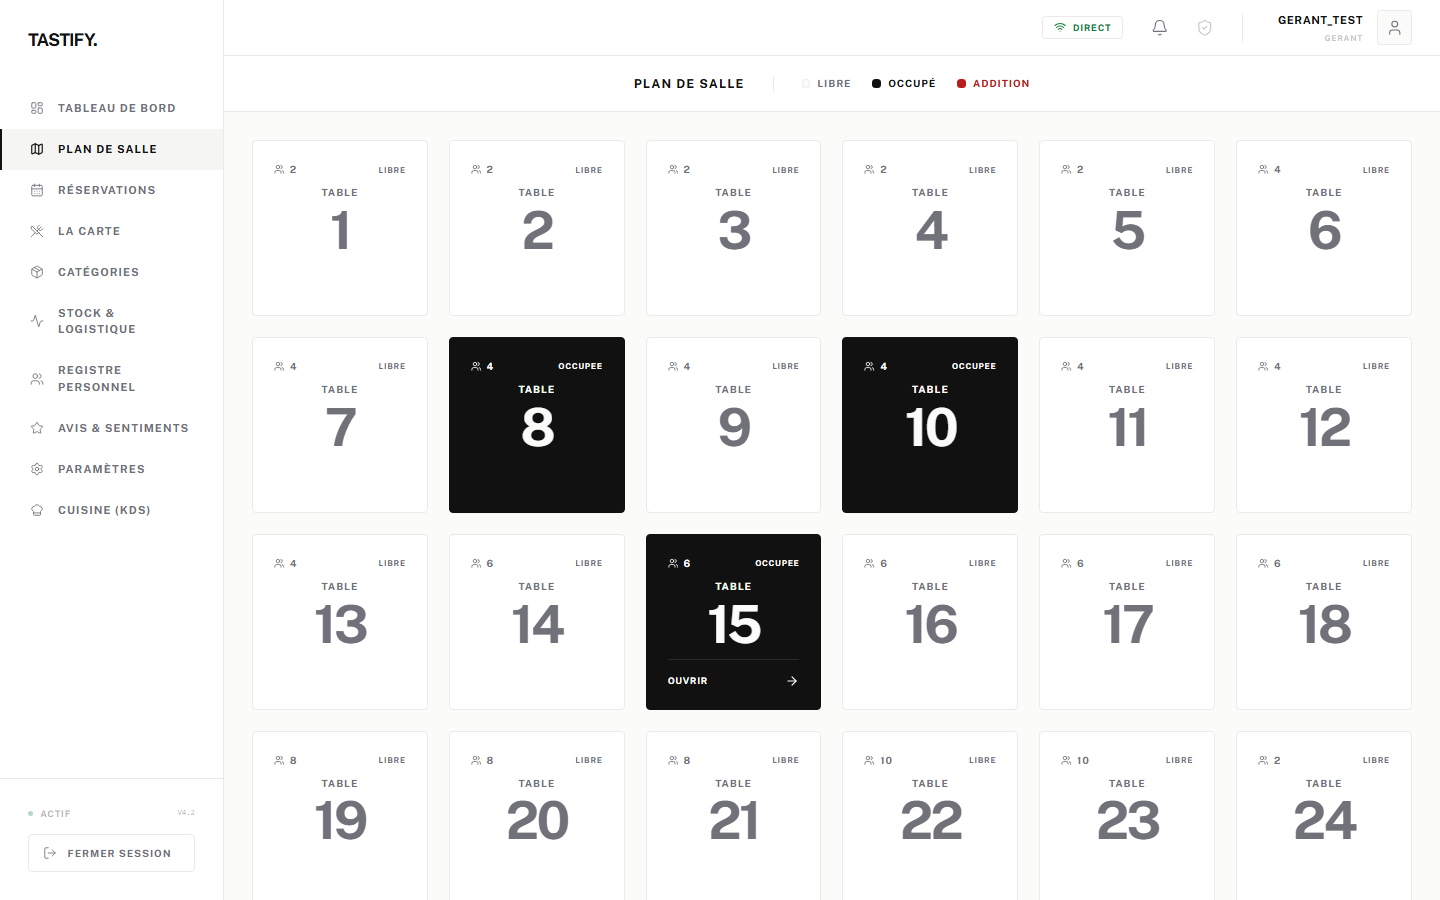
\includegraphics[width=0.95\textwidth]{capture_salle.png}
\caption{Interface serveur : plan de salle}
\label{fig:capture-salle}
\end{figure}

La figure~\ref{fig:capture-salle} montre l'espace utilisé par le serveur pour visualiser les tables, leurs statuts et l'accès à la prise de commande.

\begin{figure}[H]
\centering
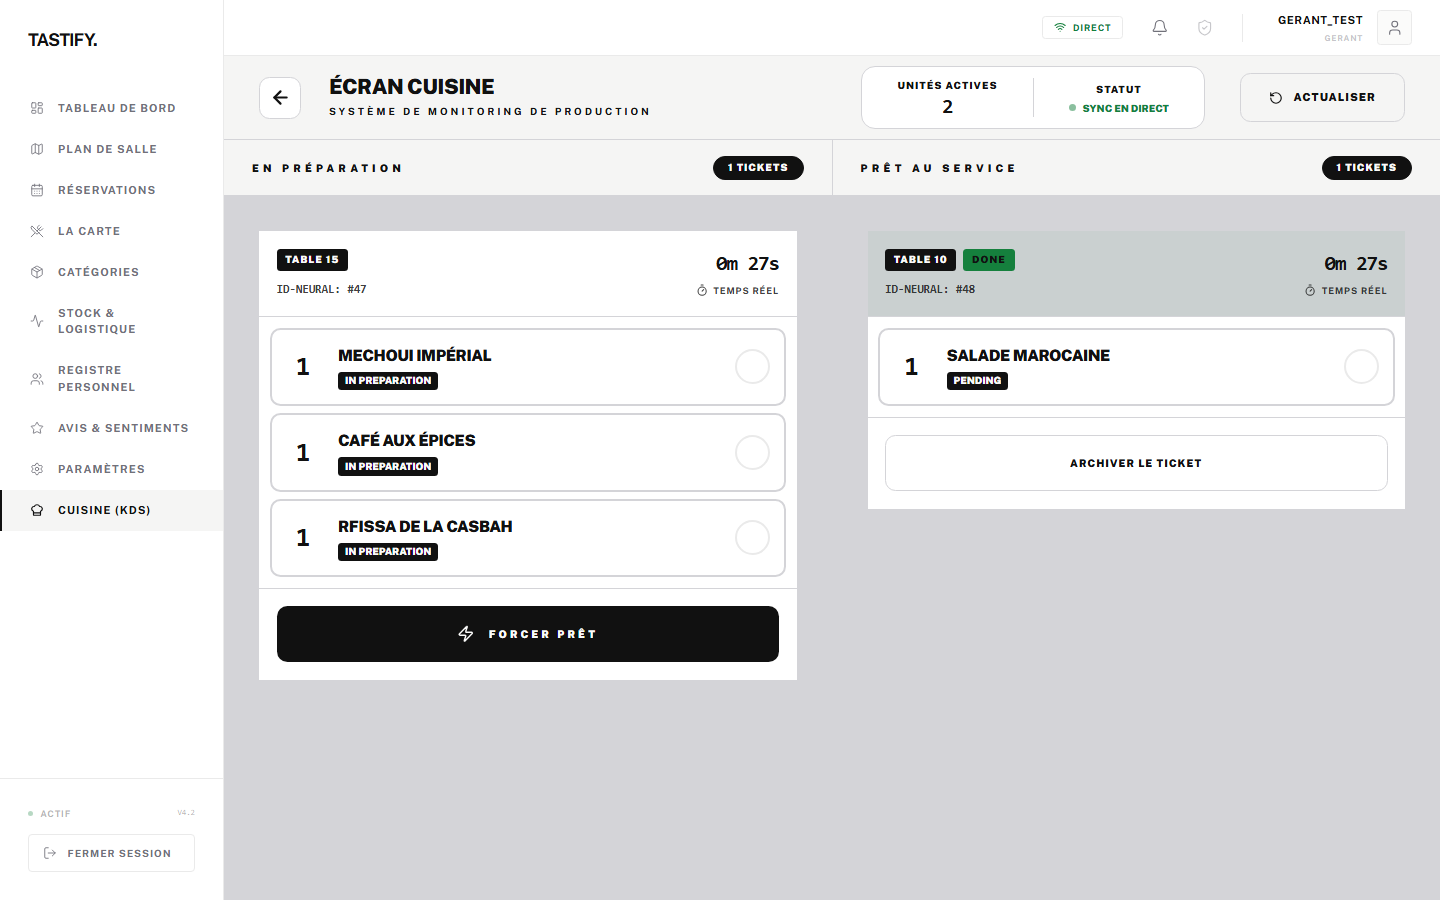
\includegraphics[width=0.95\textwidth]{capture_kds.png}
\caption{Kitchen Display System côté cuisine}
\label{fig:capture-kds}
\end{figure}

La figure~\ref{fig:capture-kds} met en évidence l'écran cuisine, conçu pour suivre les commandes et mettre à jour les statuts de préparation.

\begin{figure}[H]
\centering
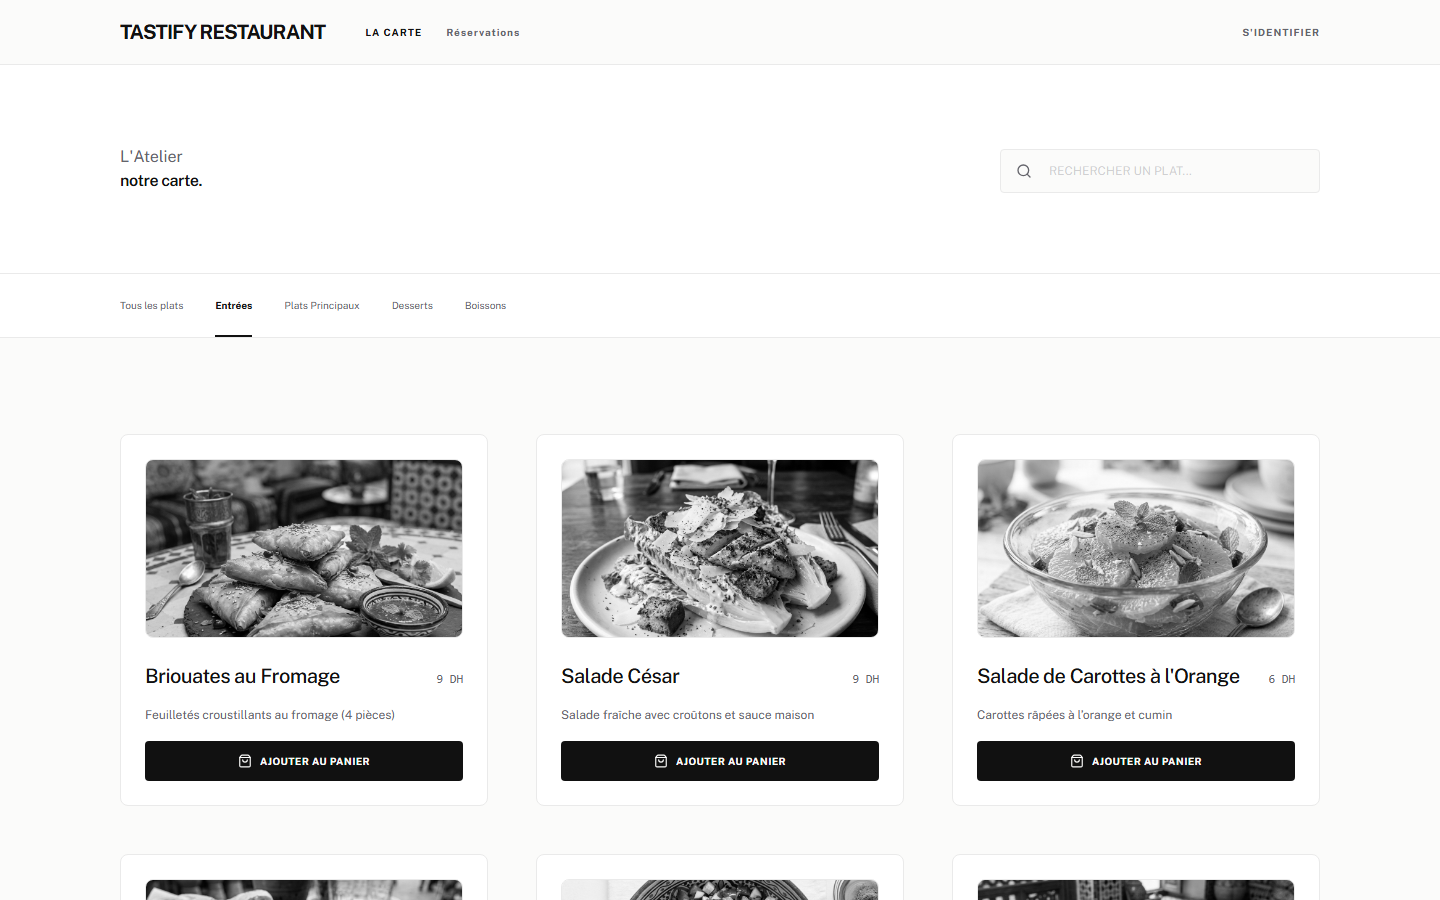
\includegraphics[width=0.95\textwidth]{capture_client.png}
\caption{Portail client : consultation du menu}
\label{fig:capture-client}
\end{figure}

La figure~\ref{fig:capture-client} présente le menu public consulté par les clients, avec les informations nécessaires pour choisir les plats disponibles.

\begin{figure}[H]
\centering
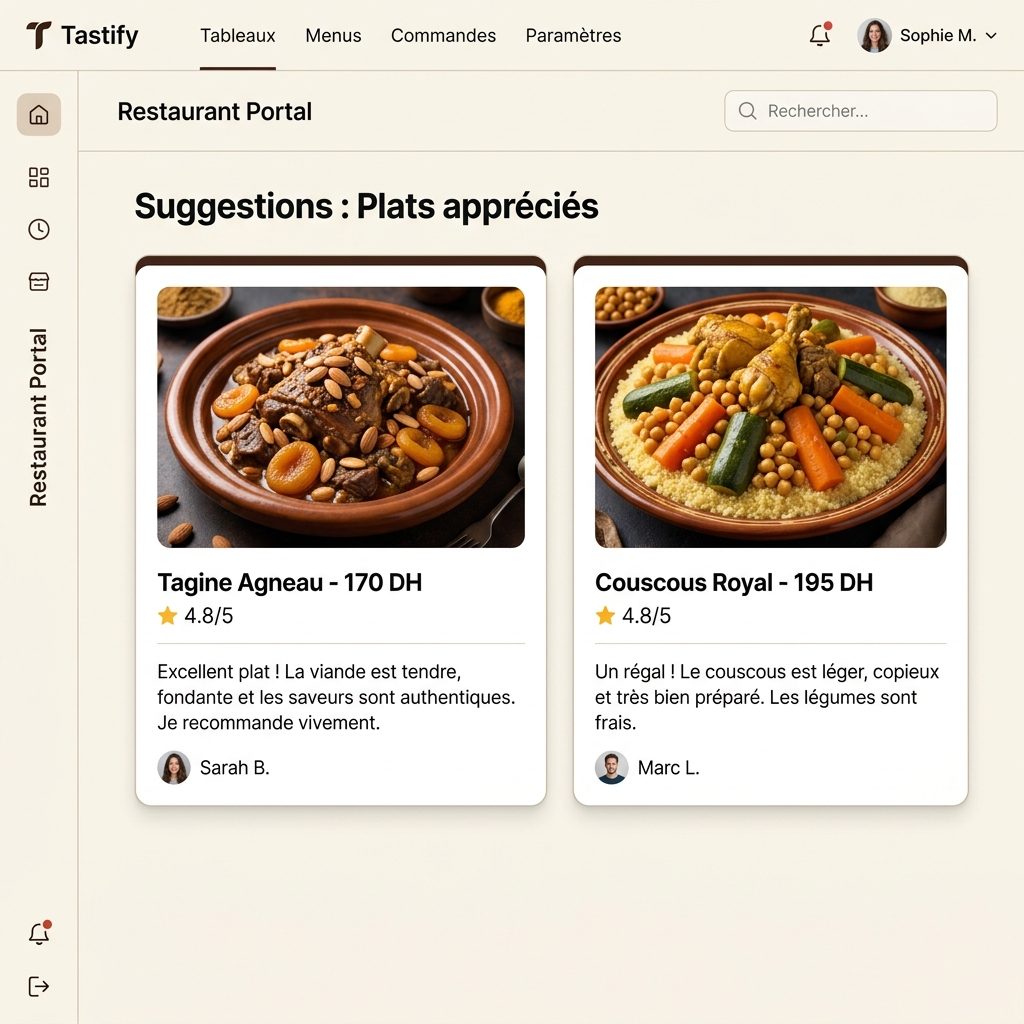
\includegraphics[width=0.95\textwidth]{capture_recommandations.png}
\caption{Portail client : plats recommandés classés selon les avis positifs}
\label{fig:capture-recommandations}
\end{figure}

La figure~\ref{fig:capture-recommandations} montre le résultat attendu côté client : les suggestions remontent les plats les mieux évalués par l'analyse de sentiment, avant les plats disposant de moins d'avis positifs.

Les figures~\ref{fig:capture-dashboard}, \ref{fig:capture-salle}, \ref{fig:capture-kds}, \ref{fig:capture-client} et \ref{fig:capture-recommandations} couvrent cinq espaces du projet : pilotage, salle, cuisine, menu et suggestions clients.

\begin{figure}[H]
\centering
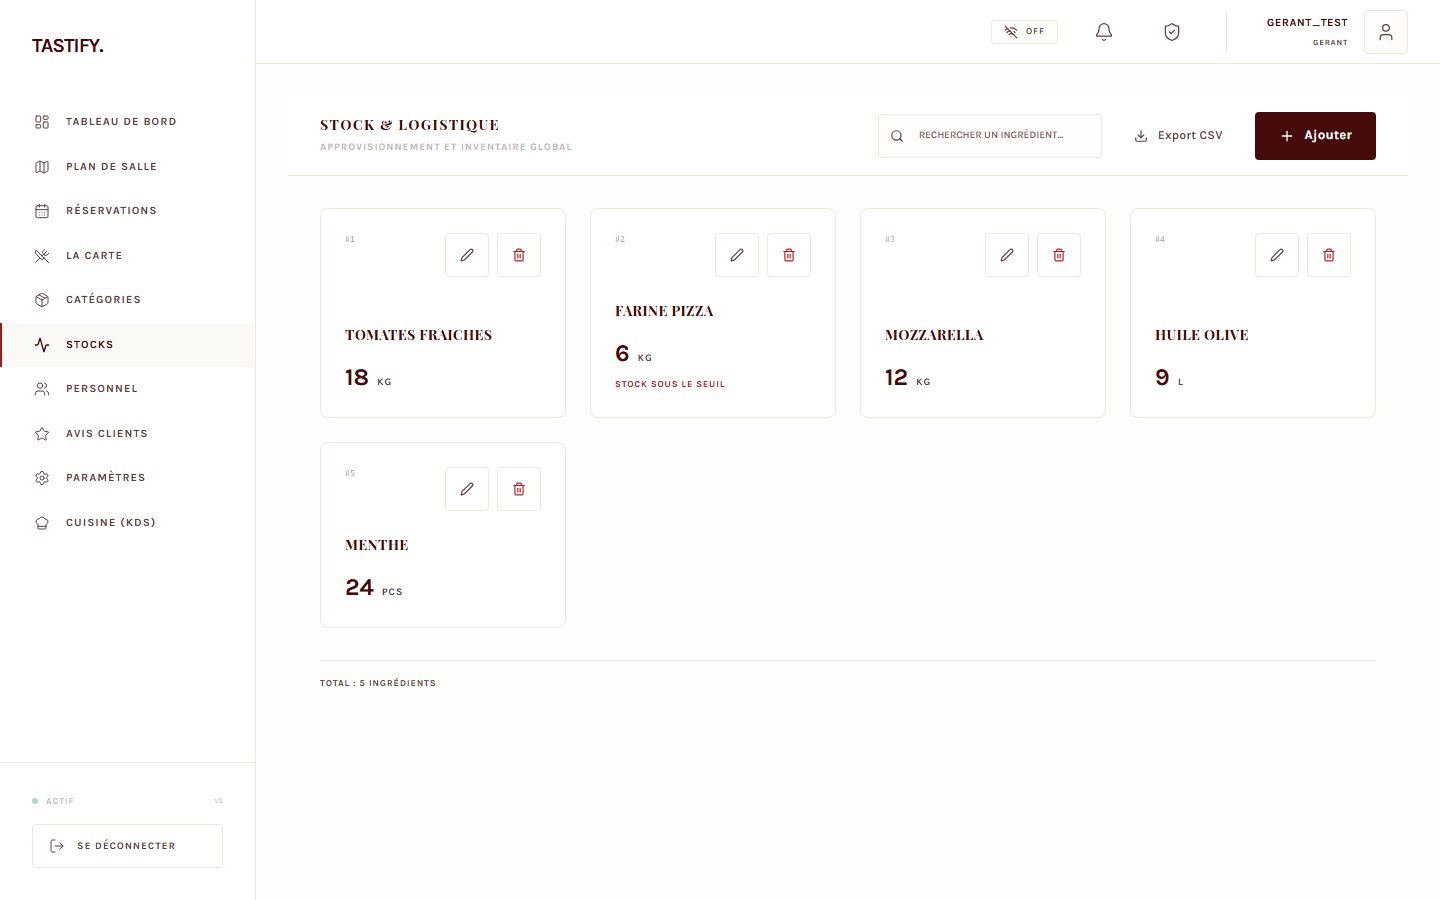
\includegraphics[width=0.95\textwidth]{capture_stock_admin.png}
\caption{Back-office : gestion du stock et alertes d'ingrédients}
\label{fig:capture-stock-admin}
\end{figure}

La figure~\ref{fig:capture-stock-admin} montre le suivi des ingrédients et des alertes, utilisé pour anticiper les ruptures de stock.

\begin{figure}[H]
\centering
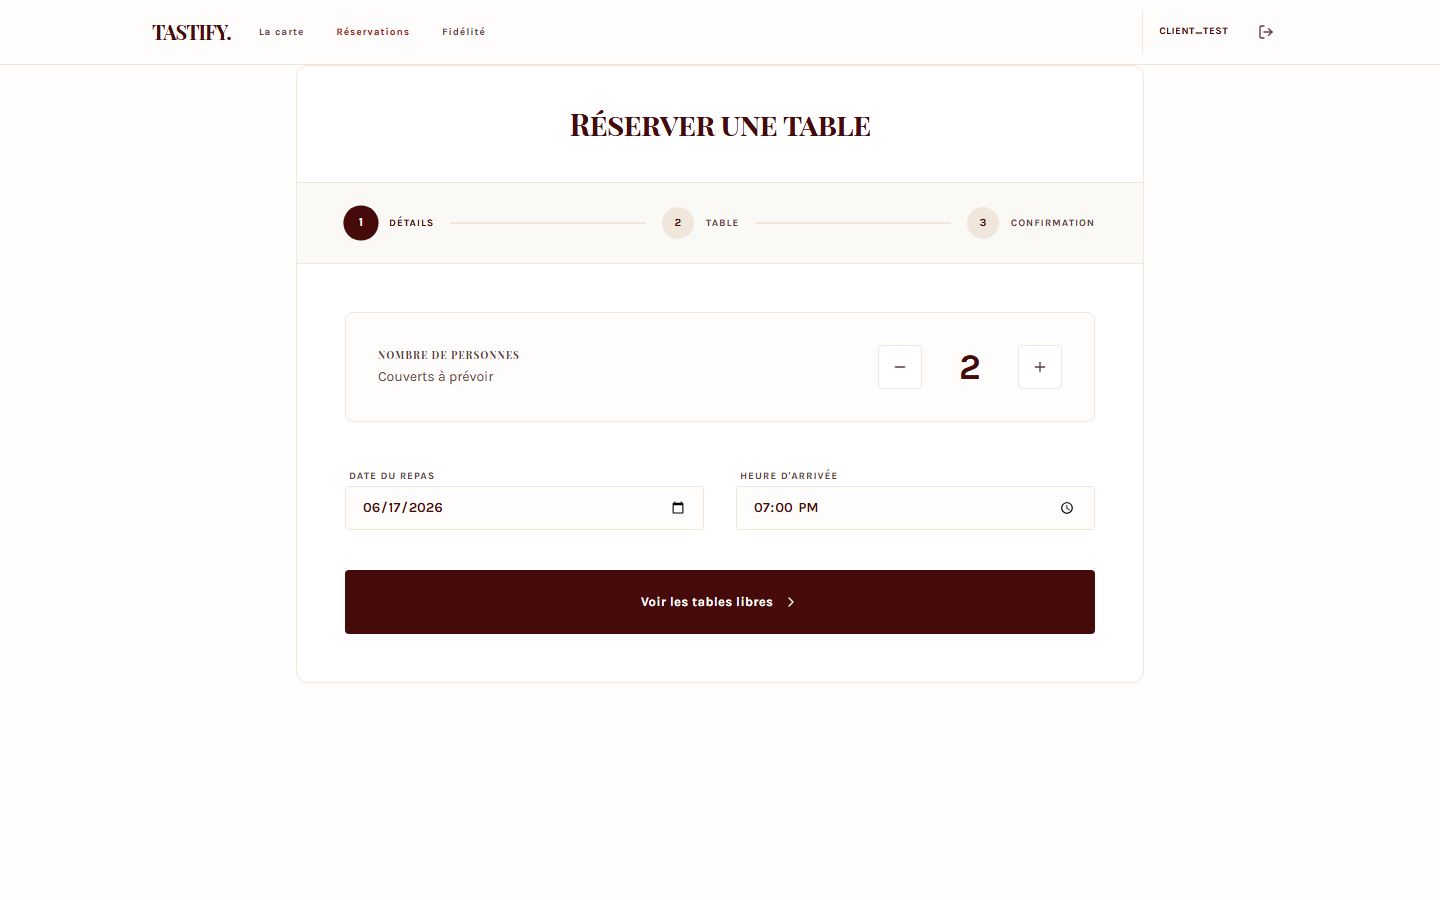
\includegraphics[width=0.95\textwidth]{capture_reservation_client.png}
\caption{Portail client : réservation d'une table}
\label{fig:capture-reservation-client}
\end{figure}

La figure~\ref{fig:capture-reservation-client} illustre le parcours de réservation côté client, depuis le choix des informations jusqu'à la demande envoyée au restaurant.

\begin{figure}[H]
\centering
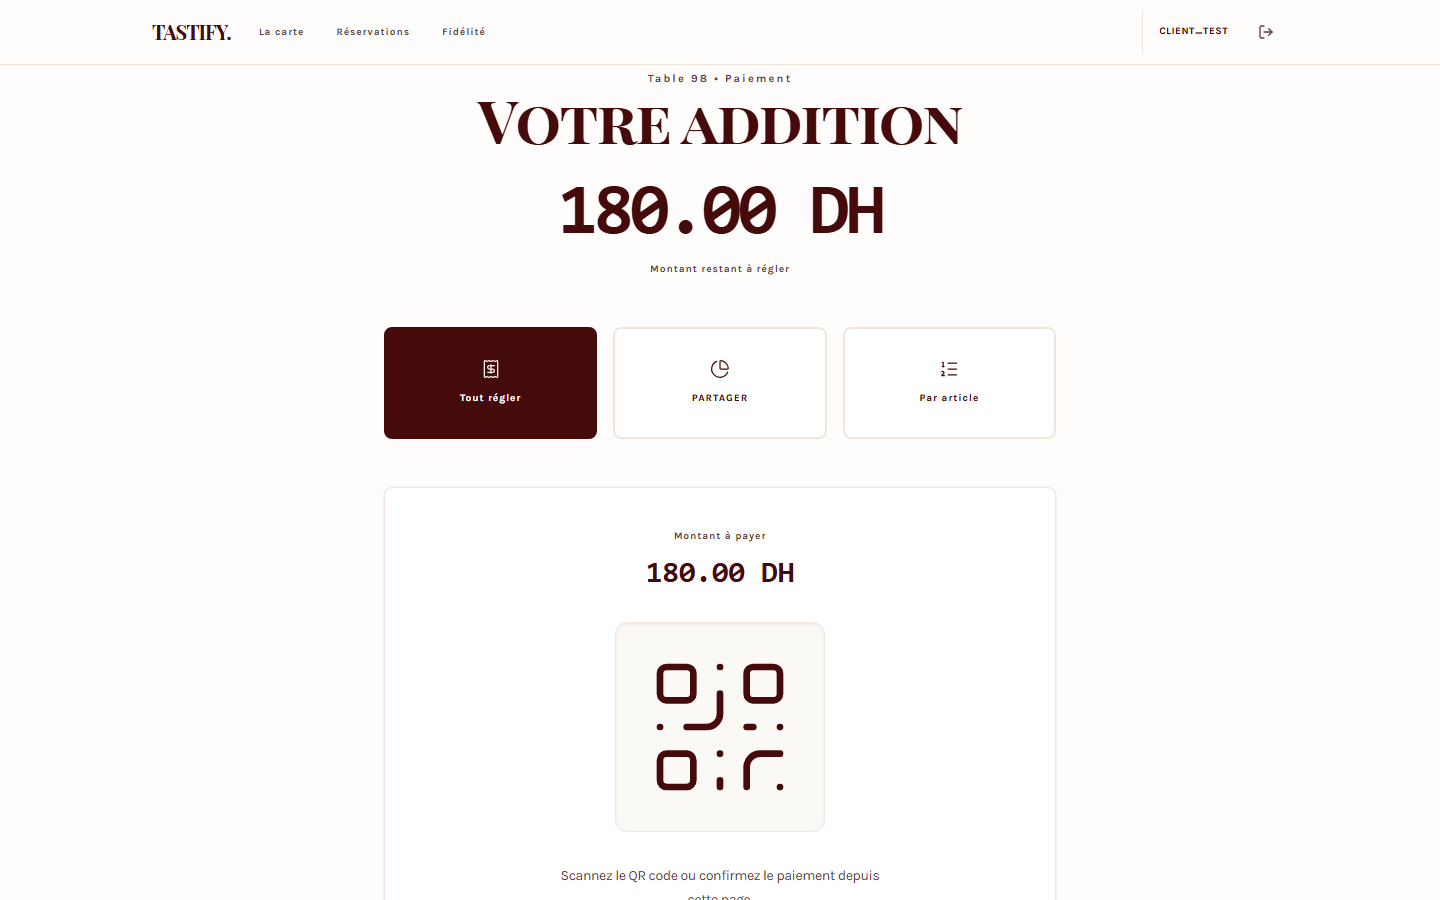
\includegraphics[width=0.95\textwidth]{capture_checkout_payment.png}
\caption{Portail client : paiement et partage de l'addition}
\label{fig:capture-checkout-payment}
\end{figure}

La figure~\ref{fig:capture-checkout-payment} présente l'étape de paiement, y compris la logique de contribution ou de partage de l'addition.

\begin{figure}[H]
\centering
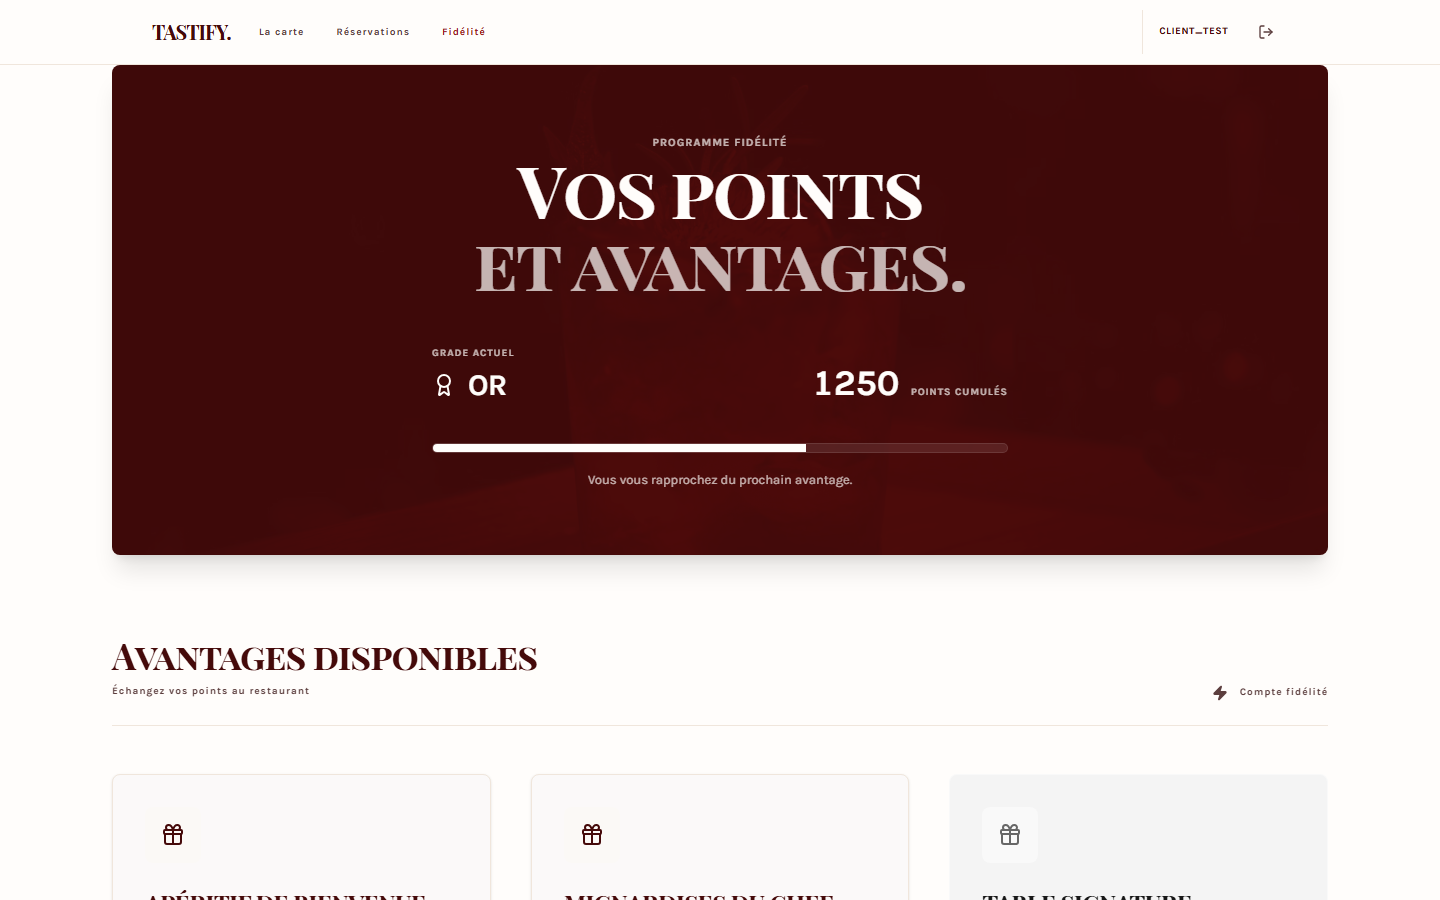
\includegraphics[width=0.95\textwidth]{capture_loyalty_client.png}
\caption{Portail client : fidélité, points et récompenses}
\label{fig:capture-loyalty-client}
\end{figure}

La figure~\ref{fig:capture-loyalty-client} montre l'espace fidélité, où le client consulte ses points, son niveau et les récompenses disponibles.

\begin{figure}[H]
\centering
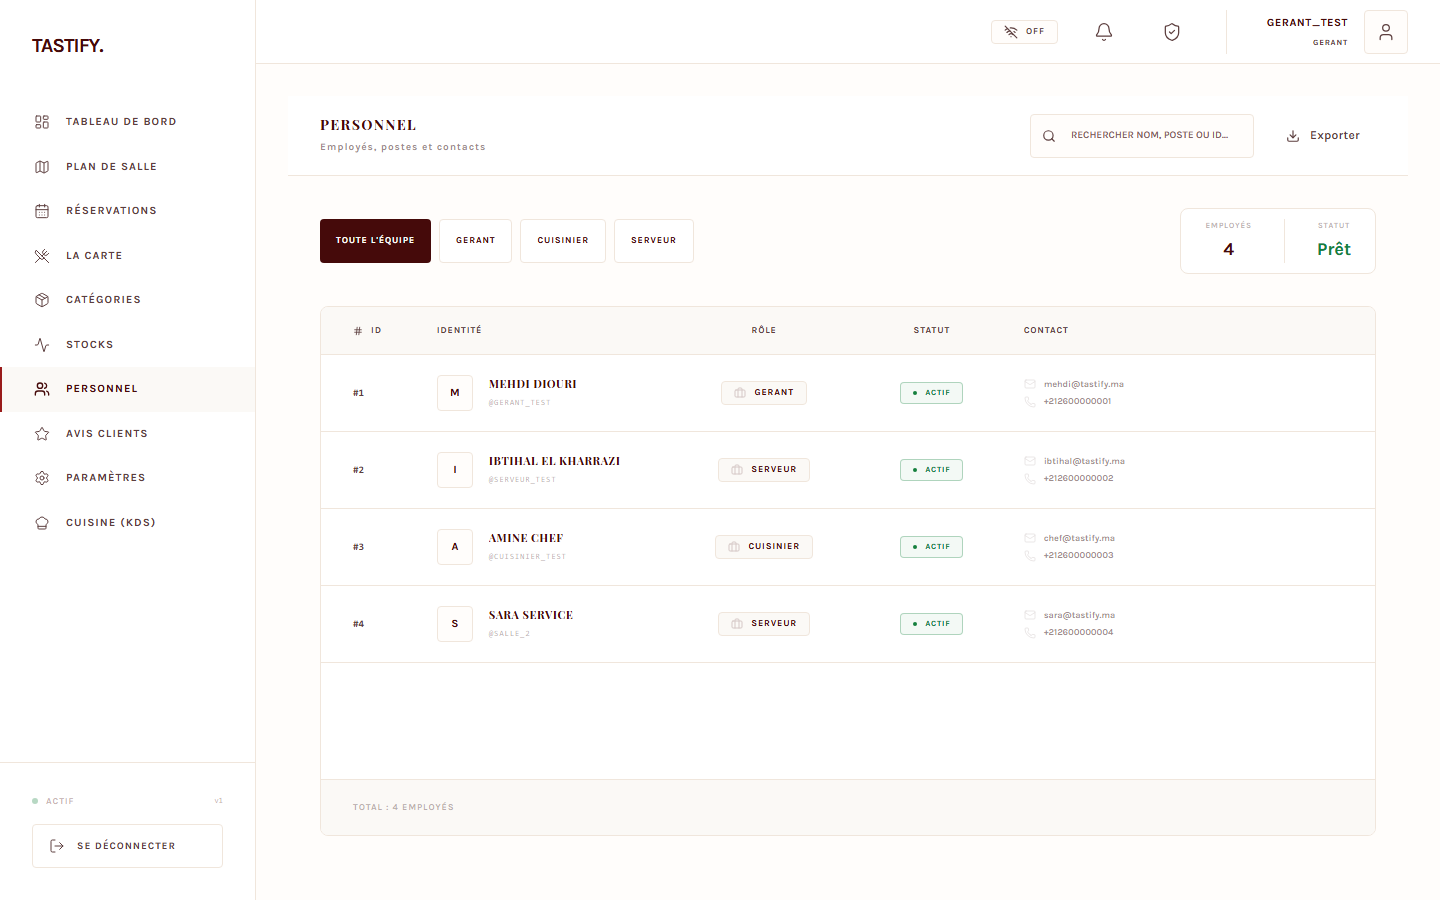
\includegraphics[width=0.95\textwidth]{capture_hr_admin.png}
\caption{Back-office : gestion des ressources humaines}
\label{fig:capture-hr-admin}
\end{figure}

La figure~\ref{fig:capture-hr-admin} illustre la partie ressources humaines du back-office, dédiée au suivi des employés et des informations associées.

Avec les captures d'avis et de sentiment du chapitre~\ref{chap:sentiment}, le rapport documente les parcours essentiels : authentification staff, pilotage, salle, cuisine, portail client, réservation, paiement, fidélité, stocks, avis et ressources humaines.

\section{Déploiement Docker Compose}
Le fichier \code{docker-compose.yml} orchestre les services de développement : base de données, Redis, backend, worker, beat, back-office et portail client.

\begin{figure}[H]
\centering
\fbox{\begin{minipage}{0.94\textwidth}
\centering
\schemaNode{\pathcode{docker-compose.yml}\\orchestration}
\schemaArrow
\schemaNode{\code{db}\\MySQL}
\schemaArrow
\schemaNode{\code{redis}\\cache et broker}

\vspace{0.45cm}

\schemaNode{\code{backend}\\Daphne}
\schemaArrow
\schemaNode{\code{celery-worker}\\\code{celery-beat}}
\schemaArrow
\schemaNode{\pathcode{backoffice-app}\\\pathcode{client-app}}
\end{minipage}}
\caption{Organisation du déploiement Docker Compose}
\label{fig:docker-compose}
\end{figure}

Cette organisation prépare un déploiement sur serveur et garde un lancement reproductible en environnement de développement.

\section*{Conclusion}
\addcontentsline{toc}{section}{Conclusion}
La réalisation de Tastify repose sur un backend Django modulaire, des API REST, des WebSocket, des tâches asynchrones, deux frontends React et Docker Compose. Ces choix répondent aux besoins métier formulés dans les chapitres précédents.

\chapter{Tests, validation, limites et perspectives}
\label{chap:tests}

\section*{Introduction}
\addcontentsline{toc}{section}{Introduction}
La validation d'un projet multi-modules doit couvrir plusieurs niveaux : backend, frontend, parcours utilisateurs, sécurité et intégration. Cette section présente les surfaces de tests observées dans le dépôt, les scénarios importants, les limites vérifiées et les perspectives d'amélioration.

\section{Stratégie de tests}
Le dépôt confirme trois familles principales de tests.

\begin{table}[H]
\centering
\caption{Familles de tests présentes dans le dépôt}
\label{tab:familles-tests}
\begin{tabularx}{\textwidth}{p{3.4cm}p{4cm}Y}
\toprule
\textbf{Famille} & \textbf{Outils} & \textbf{Objectif} \\
\midrule
Backend & pytest, pytest-django & Vérifier les modèles, permissions, API, services, signaux et tâches. \\
Frontend unitaire & Vitest, Testing Library & Tester des composants, stores et fonctions API côté React. \\
End-to-end & Playwright & Simuler des parcours utilisateur sur les applications staff et client. \\
CI et qualité & GitHub Actions, npm scripts & Automatiser lint, typecheck, build, tests et contrôles de sécurité. \\
\bottomrule
\end{tabularx}
\end{table}

Le rapport ne présente pas de résultat chiffré récent d'exécution complète, car aucune exécution globale n'a été relancée dans le cadre de la rédaction. Les commandes et suites existent, mais les résultats doivent être générés au moment de la soutenance ou de la livraison finale.

\section{Tests backend}
Les tests backend sont répartis dans les applications Django. Ils couvrent notamment :

\begin{itemize}
  \item l'authentification, les rôles et les permissions ;
  \item les réservations, conflits de créneaux et services associés ;
  \item les commandes, lignes de commande, KDS et synchronisation avec les tables ;
  \item les paiements, tokens, services et signaux ;
  \item les stocks, mouvements, seuils d'alerte et intégration avec les commandes ;
  \item les avis et l'analyse de sentiment, y compris le fallback local ;
  \item les WebSocket staff et l'autorisation des rôles internes ;
  \item la configuration restaurant et les tableaux de bord.
\end{itemize}

\begin{table}[H]
\centering
\caption{Exemples de scénarios backend critiques}
\label{tab:tests-backend}
\begin{tabularx}{\textwidth}{p{3.4cm}Y}
\toprule
\textbf{Domaine} & \textbf{Scénario à valider} \\
\midrule
Avis & Un client crée un avis, une tâche Celery est déclenchée et le résultat d'analyse est enregistré. \\
Sentiment & Hugging Face renvoie un label ; si l'API échoue, le fallback local produit un résultat. \\
RBAC & Un client ne peut pas accéder aux actions réservées au gérant ou au staff. \\
KDS & Une ligne de commande passe par les statuts attendus et reste visible côté cuisine. \\
Stock & Une commande peut déclencher une consommation d'ingrédients selon les recettes. \\
Paiement & Un paiement valide réconcilie la commande sans montant nul ou négatif. \\
Réservation & Deux réservations incompatibles sur la même table et le même créneau sont évitées. \\
\bottomrule
\end{tabularx}
\end{table}

\section{Tests frontend et end-to-end}
Les deux frontends possèdent des configurations Vitest et Playwright. Les tests end-to-end couvrent des parcours publics, authentifiés et inter-applications.

\begin{table}[H]
\centering
\caption{Parcours frontend à valider}
\label{tab:tests-frontend}
\begin{tabularx}{\textwidth}{p{3.4cm}Y}
\toprule
\textbf{Application} & \textbf{Parcours attendus} \\
\midrule
Back-office & Connexion staff, tableau de bord, menu, catégories, plan de salle, prise de commande, KDS, réservations, stocks, RH, avis, paramètres. \\
Portail client & Accueil, menu public, inscription, connexion, réservation, compte, panier, paiement, contact et fidélité. \\
Cross-app & Une réservation ou une commande côté client doit se refléter dans le back-office lorsque le scénario le prévoit. \\
Accessibilité & Navigation clavier, libellés, états d'erreur, pages not found et mode hors ligne. \\
\bottomrule
\end{tabularx}
\end{table}

\section{Validation de l'analyse de sentiment}
La validation minimale de la fonctionnalité sentiment doit couvrir les scénarios suivants :

\begin{enumerate}
  \item avis positif non arabe avec réponse Hugging Face de type \code{5 stars} ;
  \item avis négatif non arabe avec réponse \code{1 star} ;
  \item commentaire arabe routé vers \pathcode{moussaKam/MARBERT-sentiment} ;
  \item indisponibilité Hugging Face entraînant l'utilisation de \pathcode{mots-cles-simple} ;
  \item commentaire vide ne créant pas d'analyse ;
  \item agrégation correcte des labels dans le tableau de bord.
\end{enumerate}

Ces scénarios sont importants car ils testent à la fois la logique métier, l'appel externe, la normalisation des labels, la persistance et l'exploitation analytique.

\section{Tests de charge}
Le dépôt contient une configuration \code{load-tester} dans \code{docker-compose.ci.yml}, qui référence \code{scripts/locustfile.py}. Cependant, ce fichier n'est pas présent dans l'arborescence analysée. Il serait donc incorrect de présenter des résultats Locust comme réalisés.

La conclusion rigoureuse est la suivante : une campagne de charge est prévue dans l'architecture de test, mais elle doit être complétée par un fichier Locust effectif, puis exécutée pour produire des indicateurs tels que temps moyen, p95, taux d'échec et volume de requêtes.

\section{Limites du projet}
Les limites identifiées sont les suivantes :

\begin{itemize}
  \item le projet reste un prototype académique et ne fournit pas de données de production ;
  \item l'analyse de sentiment n'est pas évaluée sur un corpus d'avis Tastify annoté manuellement ;
  \item le fallback local de sentiment est volontairement simple ;
  \item la recommandation de plats n'est pas un modèle IA personnalisé complet ;
  \item la prévision de stock semble reposer sur des règles ou moyennes simples, pas sur un modèle statistique avancé validé ;
  \item les tests de charge ne sont pas exploitables tant que \code{scripts/locustfile.py} est absent ;
  \item les informations administratives dépendant de l'établissement doivent être vérifiées avant le dépôt officiel.
\end{itemize}

\section{Perspectives}
Plusieurs améliorations peuvent être envisagées :

\begin{itemize}
  \item constituer un jeu d'avis annotés pour évaluer objectivement les modèles de sentiment ;
  \item combiner commentaire et note client afin d'améliorer la fiabilité du sentiment ;
  \item remplacer ou compléter le fallback par un modèle local léger de type TF-IDF et classifieur linéaire ;
  \item améliorer la détection de langue, notamment pour le français, l'arabe dialectal et les textes mixtes ;
  \item ajouter une vraie campagne Locust et intégrer ses métriques dans la CI ;
  \item enrichir la recommandation de plats avec l'historique client et les contraintes de stock ;
  \item consolider le déploiement production avec sauvegardes, HTTPS, monitoring et rotation des secrets.
\end{itemize}

\section*{Conclusion}
\addcontentsline{toc}{section}{Conclusion}
Le dépôt présente une surface de validation sérieuse pour un PFA : tests backend, tests frontend, scénarios Playwright et CI. Les limites sont clairement identifiées et ouvrent des perspectives réalistes. Cette transparence renforce la crédibilité du rapport, car elle distingue ce qui est implémenté, ce qui est prévu et ce qui reste à prouver.

\chapter*{Conclusion générale}
\addcontentsline{toc}{chapter}{Conclusion générale}
\label{chap:conclusion}

Tastify a permis de concevoir une application web dédiée à la gestion d'un restaurant. Le périmètre réalisé couvre les modules attendus pour ce type de projet : menu, tables, commandes, cuisine, stocks, ressources humaines, réservations, paiements, fidélité, avis clients, tableaux de bord et configuration.

Sur le plan technique, le projet repose sur Django REST Framework, MySQL, Redis, Celery, Django Channels, deux applications React et Docker Compose. Cette architecture répond à un besoin simple : faire circuler l'information entre les acteurs du restaurant sans mélanger les responsabilités. Le backend porte la logique métier, l'interface staff sert les rôles internes et le portail client garde son propre usage.

L'analyse de sentiment apporte une valeur utile au projet. Elle transforme les commentaires clients en indicateurs suivis par le gérant. Le rapport a présenté cette fonctionnalité en précisant les modèles utilisés, le secours local par mots-clés, les données exploitées, la conversion des labels et les limites de validation.

Le projet atteint un périmètre solide pour un PFA full-stack : les modules principaux sont reliés, les interfaces sont exploitables, les tests automatisés valident une large partie du socle et les choix techniques sont documentés. Les prochaines priorités relèvent donc de l'industrialisation : évaluation quantitative du sentiment, tests de charge exploitables, recommandation de plats plus avancée, prévisions de stock enrichies et déploiement de production renforcé.

Tastify constitue donc une solution cohérente et défendable dans le cadre d'un Projet de Fin d'Année. Il montre la capacité à concevoir un système full-stack réaliste, à relier plusieurs modules métier, à intégrer du temps réel et des tâches asynchrones, puis à documenter les choix techniques avec précision.

\appendix
\chapter{Annexes}
\label{chap:annexes}

\section{Schémas existants intégrés}
Le tableau~\ref{tab:schemas-integres} liste les schémas existants retenus dans le rapport.

\begin{table}[H]
\centering
\small
\caption{Schémas existants intégrés}
\label{tab:schemas-integres}
\begin{tabularx}{\textwidth}{p{3.3cm}p{3cm}Y p{3cm}}
\toprule
\textbf{Fichier} & \textbf{Emplacement} & \textbf{Légende} & \textbf{Objectif} \\
\midrule
\pathcode{figure_08.jpeg} & Chapitre~\ref{chap:conception} & Diagramme de cas d'utilisation du back-office gérant & Montrer le périmètre administratif. \\
\pathcode{figure_05.png} & Chapitre~\ref{chap:conception} & Diagramme de cas d'utilisation des modules salle et cuisine & Expliquer les interactions serveur/cuisine. \\
\pathcode{figure_02.png} & Chapitre~\ref{chap:conception} & Diagramme de cas d'utilisation du portail client & Montrer les fonctions client. \\
\pathcode{figure_03.png} & Chapitre~\ref{chap:conception} & Diagramme de classes de Tastify & Présenter les entités métier majeures en page paysage. \\
\pathcode{figure_06.png} & Page de garde & Logo Tastify & Identifier visuellement le projet. \\
\bottomrule
\end{tabularx}
\end{table}

\section{Schémas techniques créés dans le rapport}
Les schémas suivants ont été créés directement en LaTeX sous forme de diagrammes textuels. Ce ne sont pas des captures d'écran.

\begin{table}[H]
\centering
\small
\caption{Schémas techniques créés}
\label{tab:schemas-crees}
\begin{tabularx}{\textwidth}{p{3.5cm}p{3.8cm}Y}
\toprule
\textbf{Schéma} & \textbf{Emplacement} & \textbf{Contenu} \\
\midrule
Architecture fonctionnelle & Chapitre~\ref{chap:conception}, figure~\ref{fig:architecture-fonctionnelle} & Deux frontends, backend DRF, MySQL, Redis, Celery et Hugging Face. \\
Pipeline de sentiment & Chapitre~\ref{chap:sentiment}, figure~\ref{fig:pipeline-sentiment} & Création avis, tâche Celery, API Hugging Face, fallback local, stockage et dashboard. \\
Architecture technique & Chapitre~\ref{chap:realisation}, figure~\ref{fig:architecture-technique} & Ports, backend ASGI, base de données, Redis, worker et beat. \\
Séquence JWT & Chapitre~\ref{chap:realisation}, figure~\ref{fig:auth-jwt} & Connexion, vérification, access token, cookie refresh et refresh ultérieur. \\
Flux KDS & Chapitre~\ref{chap:realisation}, figure~\ref{fig:flux-kds} & Serveur, API commandes, base, Redis, KDS et cuisinier. \\
Déploiement Docker Compose & Chapitre~\ref{chap:realisation}, figure~\ref{fig:docker-compose} & Services Compose et dépendances principales. \\
\bottomrule
\end{tabularx}
\end{table}

\section{Captures intégrées dans le corps du rapport}
Les captures suivantes sont intégrées dans les chapitres de réalisation, d'analyse de sentiment et de tests. Elles ne sont plus présentées comme des éléments à ajouter ultérieurement.

\begin{table}[H]
\centering
\scriptsize
\caption{Captures placées dans le corps du rapport}
\label{tab:captures-integrees}
\begin{tabularx}{\textwidth}{p{3.8cm}p{3.2cm}Y}
\toprule
\textbf{Fichier} & \textbf{Section} & \textbf{Objectif} \\
\midrule
\pathcode{capture_login_staff.png} & Réalisation & Prouver la séparation staff et l'accès sécurisé. \\
\pathcode{capture_dashboard.png} & Réalisation & Montrer le pilotage et les indicateurs gérant. \\
\pathcode{capture_salle.png} & Réalisation & Montrer la gestion opérationnelle des tables. \\
\pathcode{capture_kds.png} & Réalisation & Montrer le suivi de préparation côté cuisine. \\
\pathcode{capture_client.png} & Réalisation & Montrer la consultation du menu côté client. \\
\pathcode{capture_stock_admin.png} & Réalisation & Illustrer le suivi des ingrédients et alertes. \\
\pathcode{capture_reservation_client.png} & Réalisation & Montrer la réservation côté client. \\
\pathcode{capture_checkout_payment.png} & Réalisation & Illustrer le paiement et le partage de l'addition. \\
\pathcode{capture_loyalty_client.png} & Réalisation & Montrer les points et récompenses. \\
\pathcode{capture_hr_admin.png} & Réalisation & Montrer les employés et la gestion RH. \\
\pathcode{capture_avis_sentiment.png} & Analyse de sentiment & Relier les avis clients au score de sentiment. \\
\pathcode{capture_test_pytest.png} & Tests & Prouver les résultats backend pytest. \\
\pathcode{capture_test_vitest.png} & Tests & Prouver les résultats Vitest des frontends. \\
\pathcode{capture_test_playwright.png} & Tests & Prouver les résultats Playwright client. \\
\pathcode{capture_test_ci.png} & Tests & Relier workflow CI et validation locale. \\
\bottomrule
\end{tabularx}
\end{table}

\section{Commandes utiles}
Les commandes ci-dessous servent de rappel pour vérifier le projet et le rapport.

{\scriptsize
\begin{verbatim}
cd docs/rapport-pfa-tastify-final
pdflatex --disable-installer -interaction=nonstopmode main.tex
bibtex main
pdflatex --disable-installer -interaction=nonstopmode main.tex
pdflatex --disable-installer -interaction=nonstopmode main.tex

docker compose up -d --build
docker compose exec backend python -m pytest
npm --prefix app/frontend/backoffice-app run test:unit
npm --prefix app/frontend/client-app run test:unit
npm --prefix app/frontend/client-app run test:e2e
\end{verbatim}
}


\bibliographystyle{plain}
\bibliography{bibliography}

\end{document}
